This chapter provides an overview of the chosen signal definitions for the analysis presented here. The signal definitions are chosen to reflect the goals of the ICARUS collaboration and the SBN Program, and are designed to be simple and robust to the imperfections in the reconstruction and simulation. An overview of the signal channels and the selections are given in Section \ref{sec:neutrino_signal_definitions}. The chapter also presents the variables used to characterize the performance of the selections (Section \ref{sec:variables_of_interest}) as well as the performance of the selections on simulation (Section \ref{sec:selection_performance}).

\subsection{Neutrino Signal Definitions and Selections}
\label{sec:neutrino_signal_definitions}

\subsubsection{Signal Channels}
\label{sec:signal_channels}

Three signal definitions are chosen to accomplish the goals described above: a $\nu_\mu$ CC 1$\mu$1$p$ channel, a $\nu_\mu$ CC 1$\mu$N$p$ channel, and a $\nu_\mu$ CC inclusive channel. In common to all three of these signal channels are a few key features:

\begin{itemize}
    \item \textbf{Containment}: The entirety of the interaction is required to be contained within a volume that is defined as \qty[mode=text]{5}{cm} from the edges of the detector in all three dimensions. This requirement ensures that the range-based energy reconstruction, which has significantly better resolution than other methods, can be applied to tracks in the final state.
    \item \textbf{Fiducial Volume}: The interaction vertex must be located within the fiducial volume of the detector, which is defined as the region \qty[mode=text]{25}{cm} from the edges of the detector in the $x$ and $y$ directions, \qty[mode=text]{30}{cm} from the upstream edge in the $z$ direction, and \qty[mode=text]{50}{cm} from the downstream edge in the $z$ direction. This requirement is motivated by the desire to avoid the reconstruction inefficiencies and biases that can arise near the edges of the detector.
    \item \textbf{Single Muon}: Each signal definition requires the presence of a single primary muon in the final state. This muon is required to have a length of at least \qty[mode=text]{50}{cm}, principally to reduce the contamination from NC interactions with a pion in the final state. This length threshold is also consistent with the proposed selection in the SBN proposal.
    \item \textbf{Proton Threshold}: Protons are required to be primary particles and to have deposited at least \qty[mode=text]{50}{MeV} of energy to count towards the final state of the interaction. This threshold is chosen to ensure that the proton is sufficiently long to be reconstructed as a track and to ensure that the proton is energetic enough to be well-separated from the muon in the final state. Interactions with one proton above threshold and one proton below threshold are classified as 1$\mu$1$p$ final states under this definition.
    \item \textbf{Other Particles}: The final state may contain additional protons, pions, and showers. These particles are required to be primary particles and to have deposited at least \qty[mode=text]{25}{MeV} of energy to be counted towards the final state of the interaction. This threshold is chosen to ensure that the particles are sufficiently energetic to be visible in the final state.
\end{itemize}

The 1$\mu$1$p$ channel requires exactly one proton above threshold in addition to the muon, while the 1$\mu$N$p$ channel requires \text{at least} one proton above threshold in addition to the muon. The $\nu_\mu$ CC inclusive channel requires only the presence of a single muon in the final state and any number of other final state particles above threshold. The structuring of these signal definitions means that the 1$\mu$1$p$ channel is a subset of the 1$\mu$N$p$ channel, which is in turn a subset of the $\nu_\mu$ CC inclusive channel. 

While the 1$\mu$1$p$ and 1$\mu$N$p$ channels are inherently more statistically limited than the $\nu_\mu$ CC inclusive channel, they provide simple final states that are well-suited to the early stages of the ICARUS physics program. The energy reconstruction for these two channels is also more precise due to the simple final state, which may be beneficial for neutrino oscillation physics measurements. Additionally, these final states are particularly low in cosmic background, especially in combination with the containment requirement. In contrast, the $\nu_\mu$ CC inclusive channel is more statistically powerful and provides a more complete picture of the detector performance due to the wider range of neutrino interaction topologies. Final states in this channel may also contain showers, the precise reconstruction of which is of significant importance for any future oscillation analysis.

\subsubsection{Additional Selections}
\label{sec:additional_selections}

In addition to the requirements described above, the following selections are applied to the reconstructed interactions to further reduce the background and improve the purity of the selected samples:

\paragraph{Flash Time:}
Each interaction is required to be matched with an optical flash detected by the PMTs that is consistent with the time of the neutrino beam spill. The association of the interaction with the flash is performed with OpT0Finder, as described in Section \ref{sec:post_processing}. This analysis targets neutrinos from the BNB, which has a spill length of \qty[mode=text]{1.6}{us}. The requirement that interactions be associated with a flash in-time with the beam provides significant background rejection of cosmic-induced interactions that are not in-time with the beam. This cut is not expected to provide significant background rejection for cosmic-induced interactions that are in-time with the beam and trigger the detector readout.

\paragraph{CRT Veto:}
Each event has a collection of PMT flashes and CRT hits. As part of the standard reconstruction chain, a matching algorithm is run to associate the CRT hits with the PMT flashes using timing information. This analysis makes use of this association by requiring that selected events have at least one flash within the beam spill window that is not matched to a CRT hit. This requirement strongly suppresses cosmic-induced interactions, and is complementary to the flash time cut discussed above in that it rejects many of the cosmic-induced interactions that are in-time with the beam. This veto uses only the Top and Side CRT subsystems, as the Bottom CRT subsystem was not fully commissioned prior to the data used in this analysis.

\subsubsection{Neutrino Sample Composition}
\label{sec:neutrino_sample_composition}
The primary sample used in this analysis to set the central value expectation for the selections is a sample of simulated neutrino interactions produced according to the predicted BNB flux and overlayed with the expected out-of-time cosmic flux. The size of this sample is $2.68 \times 10^{20}$ POT, which is more than a factor of ten larger than the recorded dataset of $1.92 \times 10^{19}$ POT for this analysis. The statistical uncertainty of this larger simulated sample is negligible for the analysis presented here. It is worth noting that the neutrinos in this sample are required to interact in the active volume of the detector. The contribution to the expected event rates from neutrinos that interact outside of the active volume is expected to be negligible and thus is not included in this analysis.

Most of the triggered events in data are due to cosmic muons in-time with the beam, which are not present in the simulated neutrino sample. Rather than attempting to model the cosmic background with a simulated dataset, the cosmic background is estimated using the off-beam dataset. This method is expected to provide a more accurate estimate of the cosmic background than a simulated dataset, which would be subject to uncertainties in the cosmic flux and the detector response to cosmic-induced interactions. The scaling of the off-beam dataset to the on-beam dataset is based on matching the number of opened trigger gates in the two datasets. Though the number of opened trigger gates is one-to-one, and therefore the number of on-beam and off-beam events is near equal, there is a limited statistical penalty due to both the smallness of the background and the ability to use the entire off-beam dataset rather than the 10\% that is used for the on-beam dataset due to blinding considerations. The on-beam dataset used in this analysis will be described in more detail in Chapter \ref{chap:data_mc_comparisons} and the uncertainty associated with the data-driven cosmic background estimate will be assessed in Chapter \ref{chap:systematics}.

\subsection{Variables of Interest}
\label{sec:variables_of_interest}

This section presents an overview of the variables used to characterize the performance of the three selections described in the preceding section. The variables are divided into three categories: interaction kinematic variables, kinematic imbalance variables, and PID variables. The distributions of these variables can be used to validate the performance of the selections and to identify potential sources of bias or inefficiency in the reconstruction and simulation. In each of the following plots, the distributions are made with truth information to show the true distributions of these variables for each of the signal channels prior to any reconstruction or selection effects. The distributions are also scaled to the recorded dataset of $1.92 \times 10^{19}$ POT to show the predicted event rates.

\subsubsection{Interaction Kinematic Variables}
\label{sec:interaction_kinematic_variables}
These variables reflect the kinematics of the neutrino interaction and the final state particles. The total energy of the interaction is a key variable for understanding the energy of the parent neutrino, while the kinematics of the final state particles can provide information about the nature of the interaction and the performance of the reconstruction. The total energy of the interaction is a necessary input to oscillation analyses. Additionally, these variables are often used in cross section measurements to probe the underlying physics of neutrino interactions. For the chosen signal definitions, there is always a single primary muon and there may be additional primary protons, pions, and showers above the energy threshold of the signal definition. 

\paragraph{Muon Kinetic Energy ($\mathbf{T_\mu}$):}
The kinetic energy of the muon as calculated using the Continuous Slowing Down Approximation (CSDA) \cite{Zyla2020} to relate the muon track length (range) to its kinetic energy. This method is typically known as ``range-based'' kinetic energy reconstruction.

\paragraph{Leading Proton Kinetic Energy ($\mathbf{T_p}$):}
The kinetic energy of the most energetic primary proton as calculated using the CSDA to relate the proton track length (range) to its energy.
    
\begin{figure}[!htb]
    \centering
    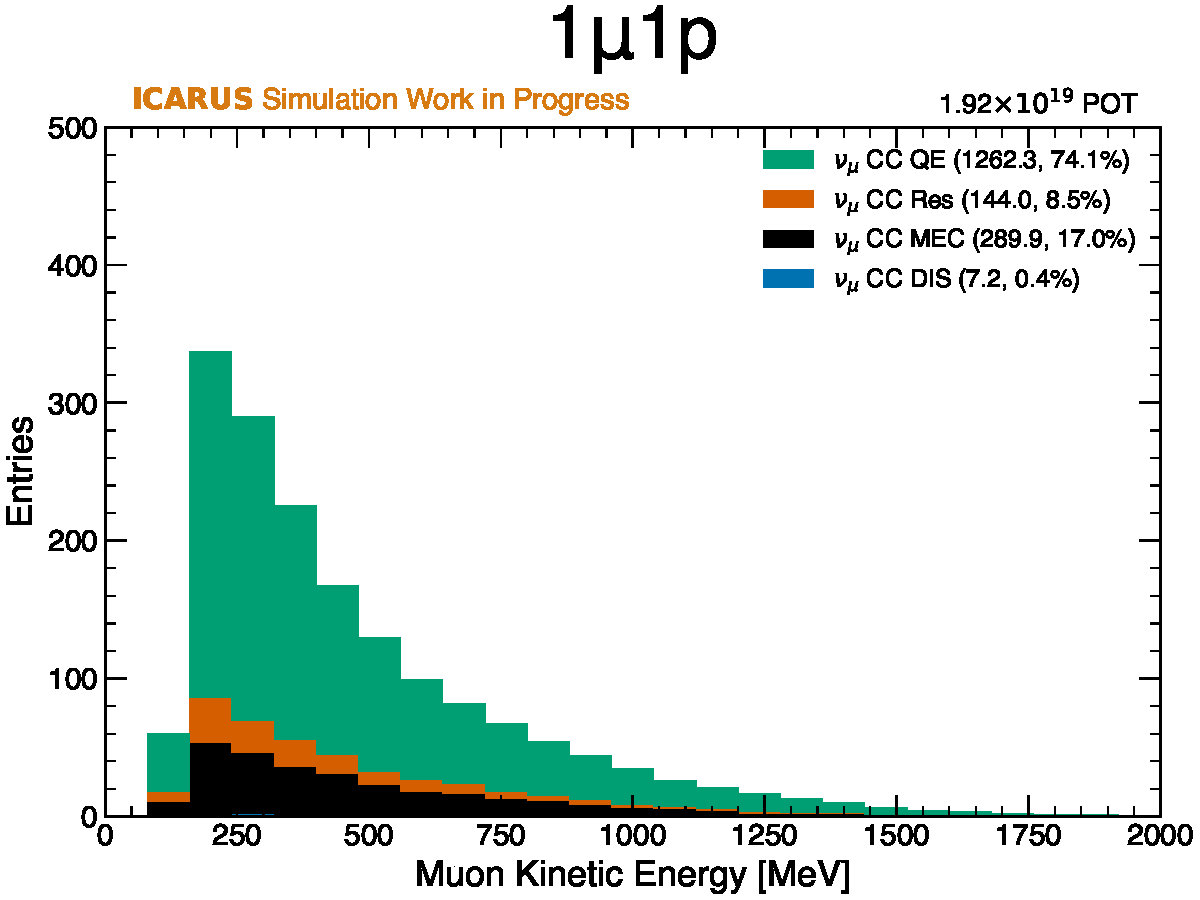
\includegraphics[width=0.48\textwidth]{figures/neutrino_selection/signal_hist1d_1mu1p_muon_ke.pdf}
    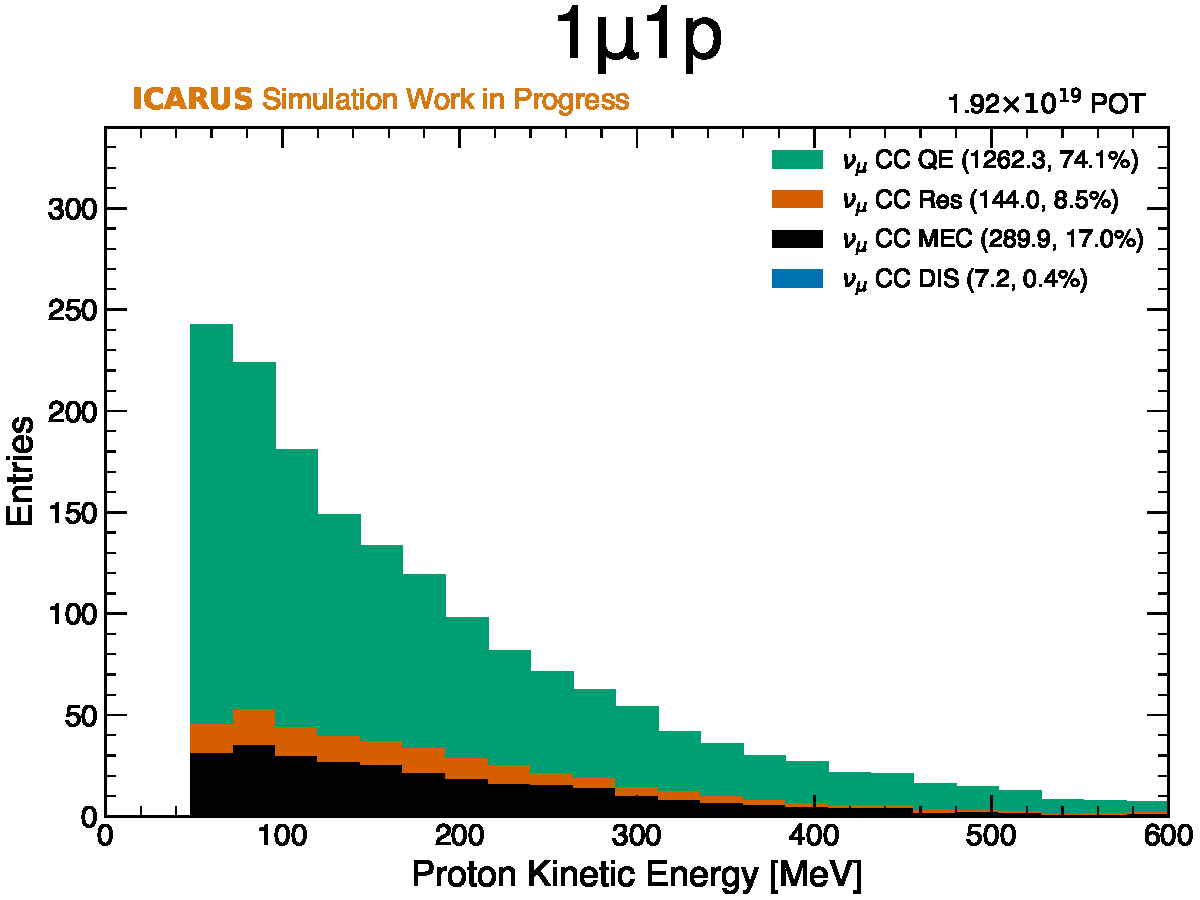
\includegraphics[width=0.48\textwidth]{figures/neutrino_selection/signal_hist1d_1mu1p_proton_ke.pdf}
    \\
    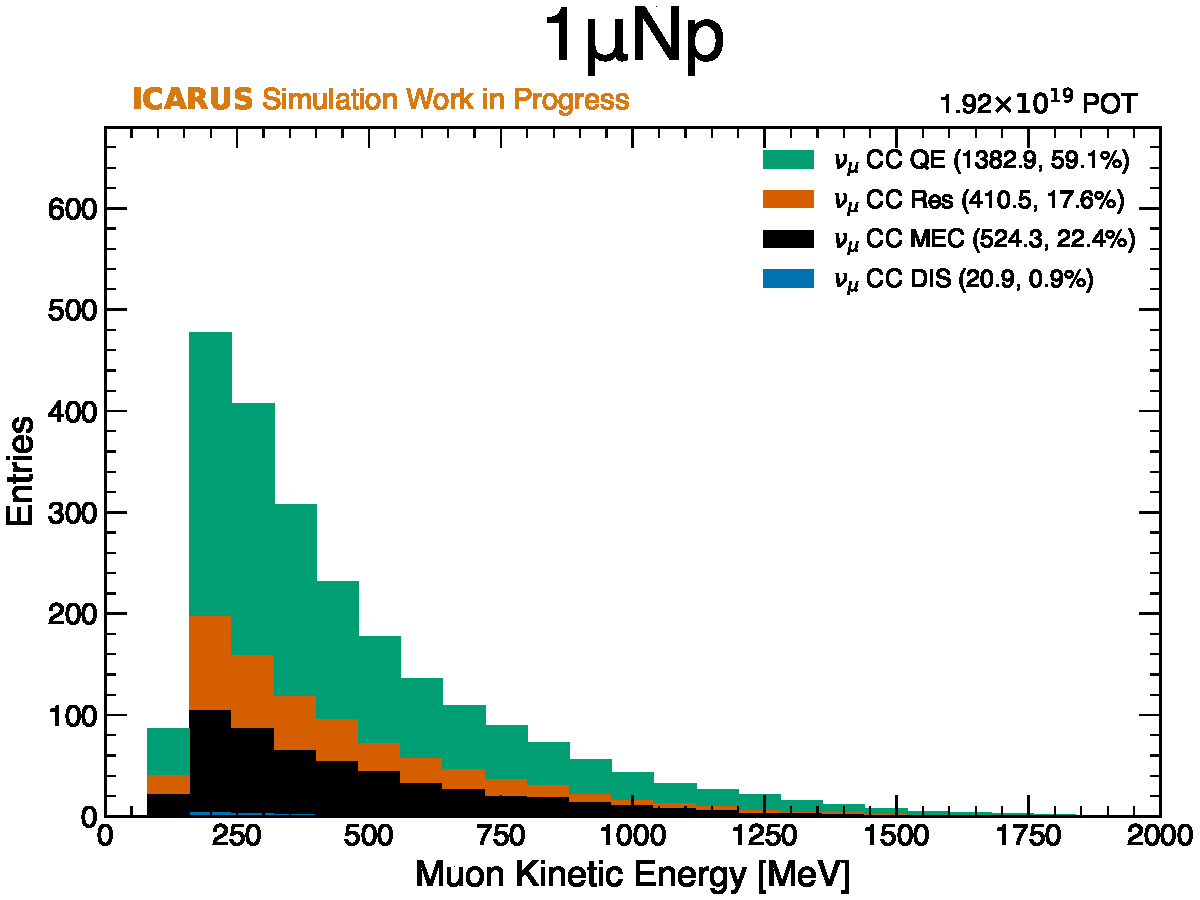
\includegraphics[width=0.48\textwidth]{figures/neutrino_selection/signal_hist1d_1muNp_muon_ke.pdf}
    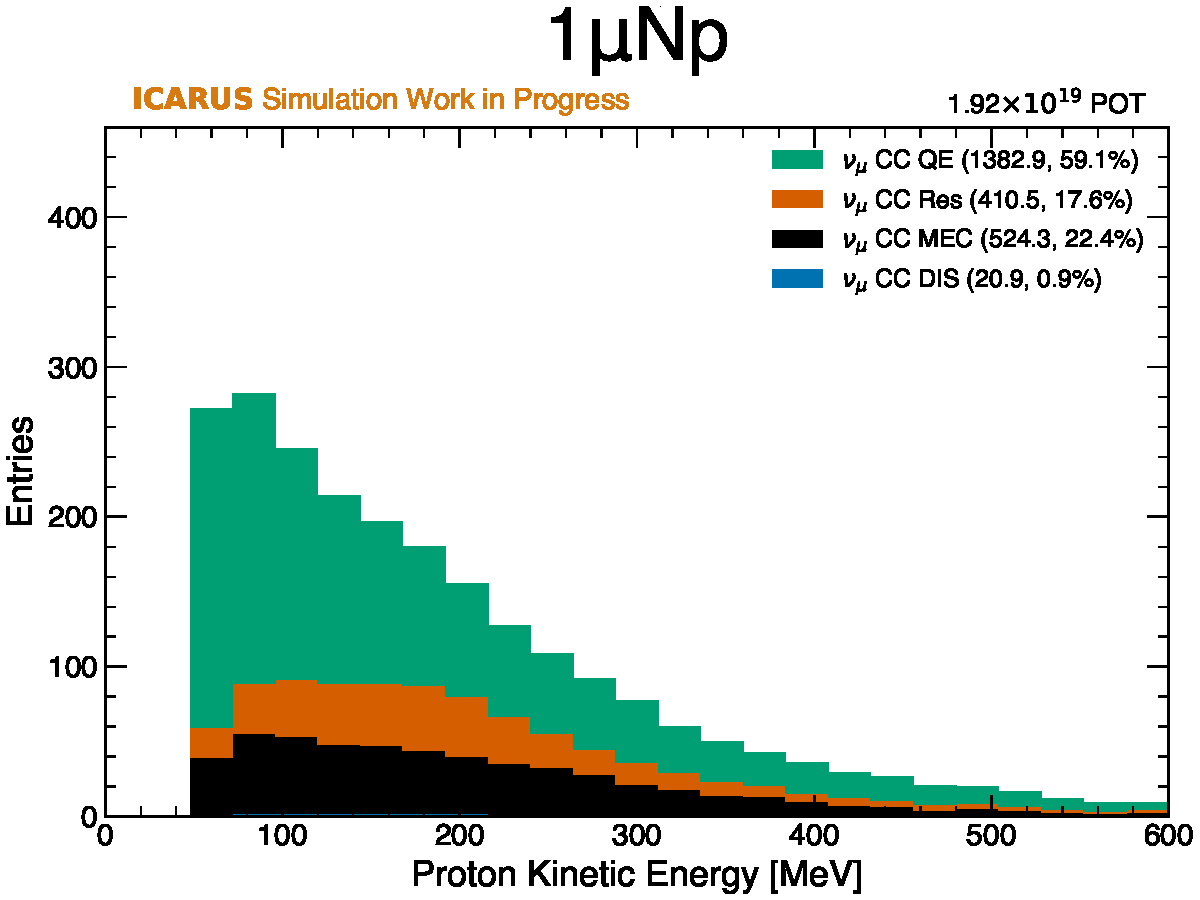
\includegraphics[width=0.48\textwidth]{figures/neutrino_selection/signal_hist1d_1muNp_proton_ke.pdf}
    \\
    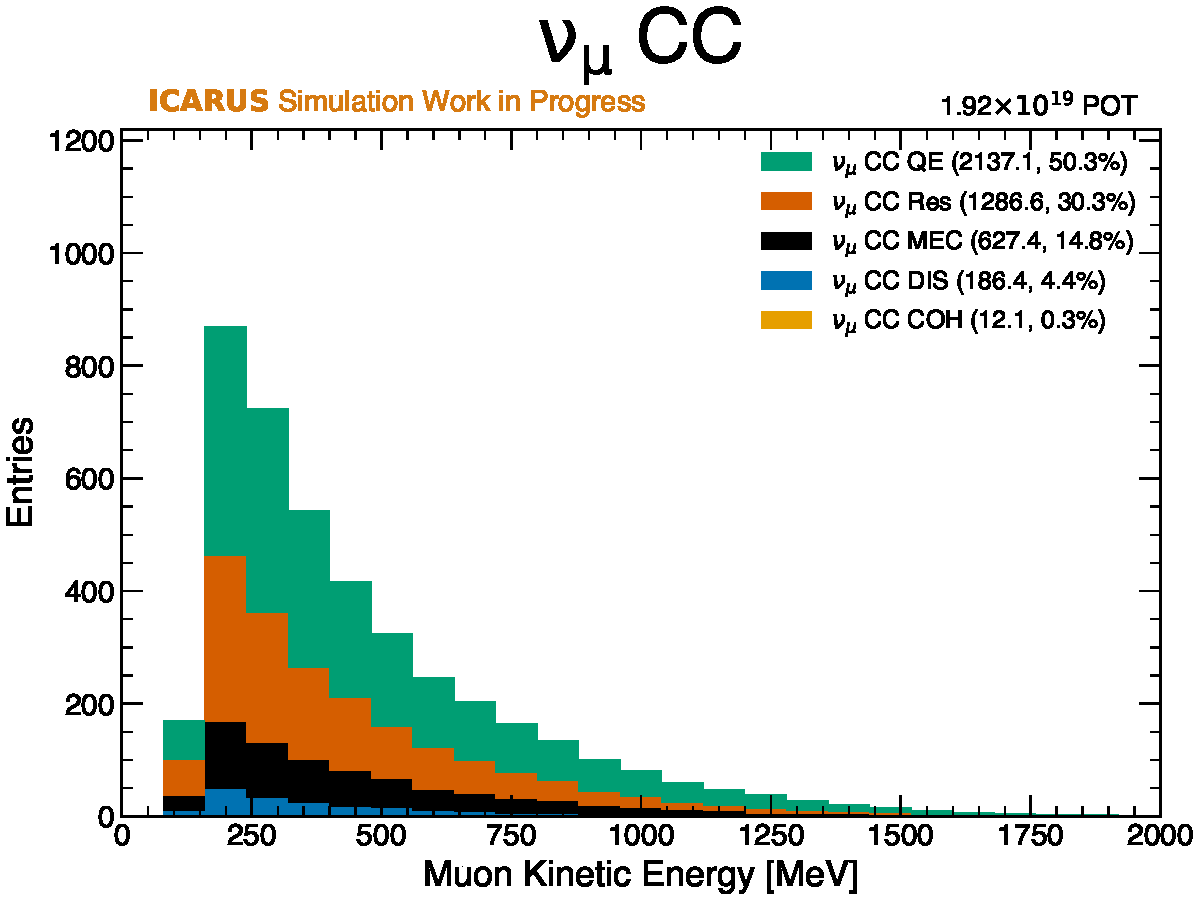
\includegraphics[width=0.48\textwidth]{figures/neutrino_selection/signal_hist1d_1muX_muon_ke.pdf}
    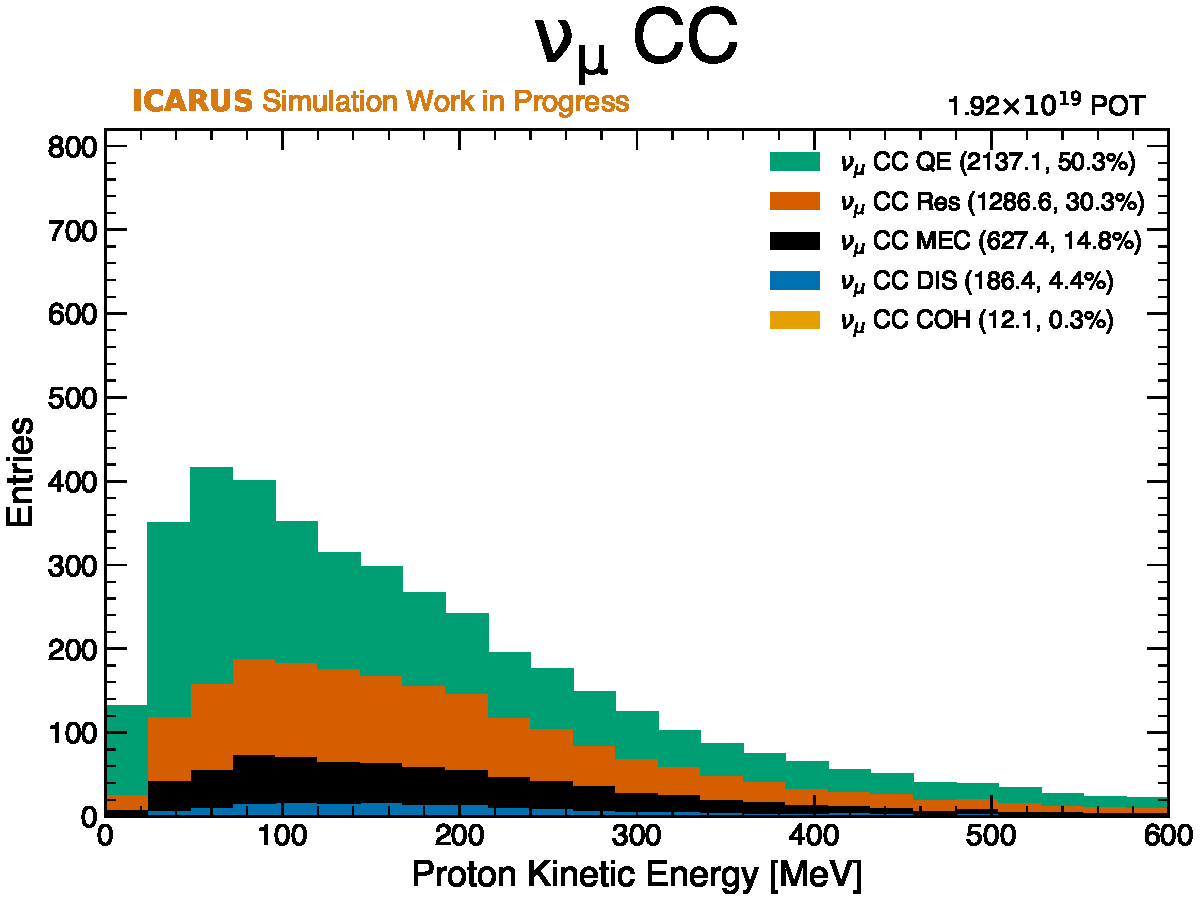
\includegraphics[width=0.48\textwidth]{figures/neutrino_selection/signal_hist1d_1muX_proton_ke.pdf}
    \caption{Kinetic energy of the muon (left) and the most energetic proton (right) for each of the three signal channels: from top to bottom $\mathrm{1\mu 1p}$, $\mathrm{1\mu Np}$, and $\nu_\mu$ CC inclusive.}
    \label{fig:muon_proton_ke}
\end{figure}

\paragraph{Interaction Visible Energy ($\mathbf{E_{vis}}$):}
The best estimate of energy deposited in the detector by the neutrino interaction. The energy deposited by primary showers are estimated by summing the deposited charge and converting it to energy using an effective constant that accounts for electron-ion recombination and shower clustering efficiency. Primary muon, pion, and proton energies are estimated using the CSDA to relate the track length to the energy deposited. In addition to the kinetic energies of the particles, the mass of the particle is also included in the energy calculation for the muon and pion, which are created rather than ejected during the interaction. Neutrons leading to recoiling protons are not currently included in the energy calculation as they are classified as secondaries and only primary particles are included for now. The interaction visible energy is therefore calculated as:
\begin{equation}
    E_{\text{vis}} = \sum_{\mathrm{Showers}} E^{calo}_{\mathrm{shower}} + \sum_{\mathrm{Muons}} E^{range}_{\mathrm{muon}} + \sum_{\mathrm{Pions}} E^{range}_{\mathrm{pion}} + \sum_{\mathrm{Protons}} T^{range}_{\mathrm{proton}}
\end{equation}

\begin{figure}[!htb]
    \centering
    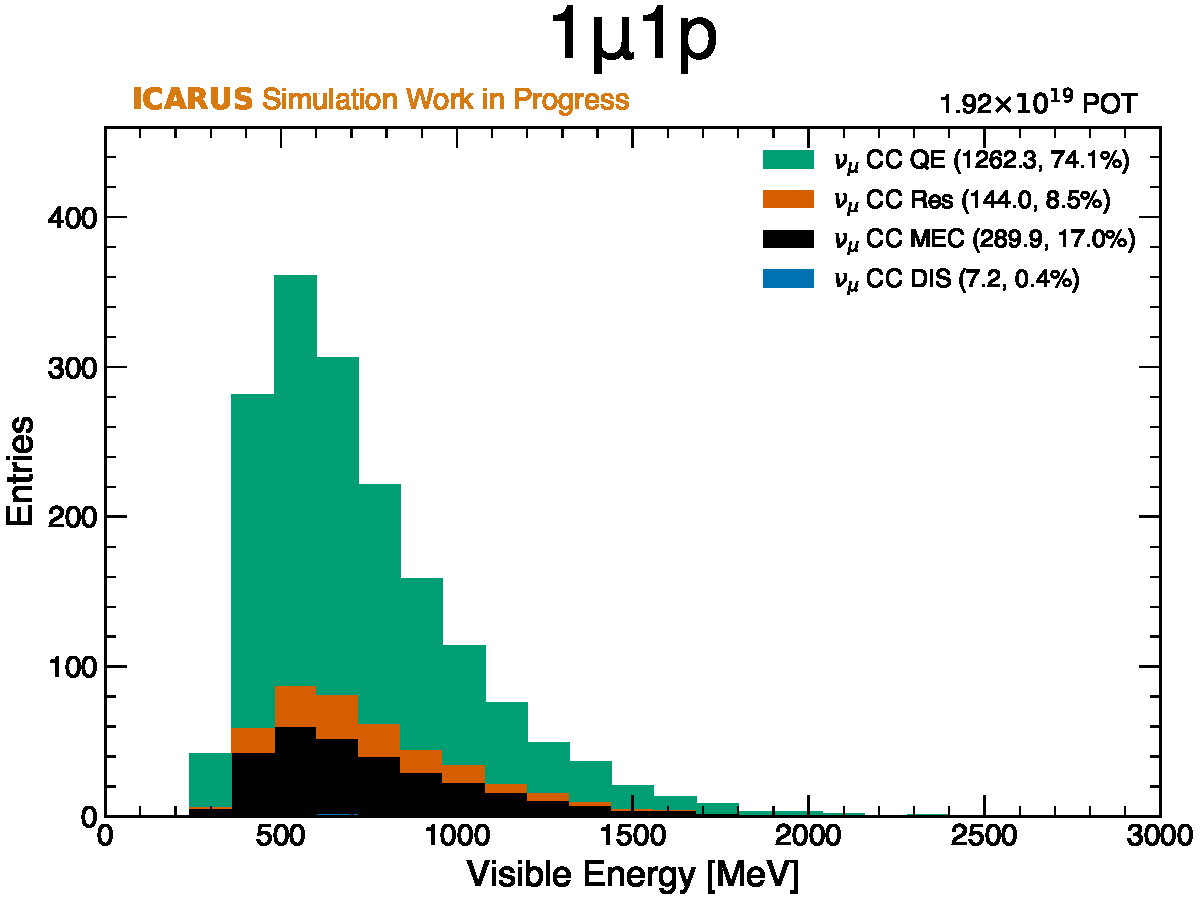
\includegraphics[width=0.48\textwidth]{figures/neutrino_selection/signal_hist1d_1mu1p_visible_energy.pdf}\\
    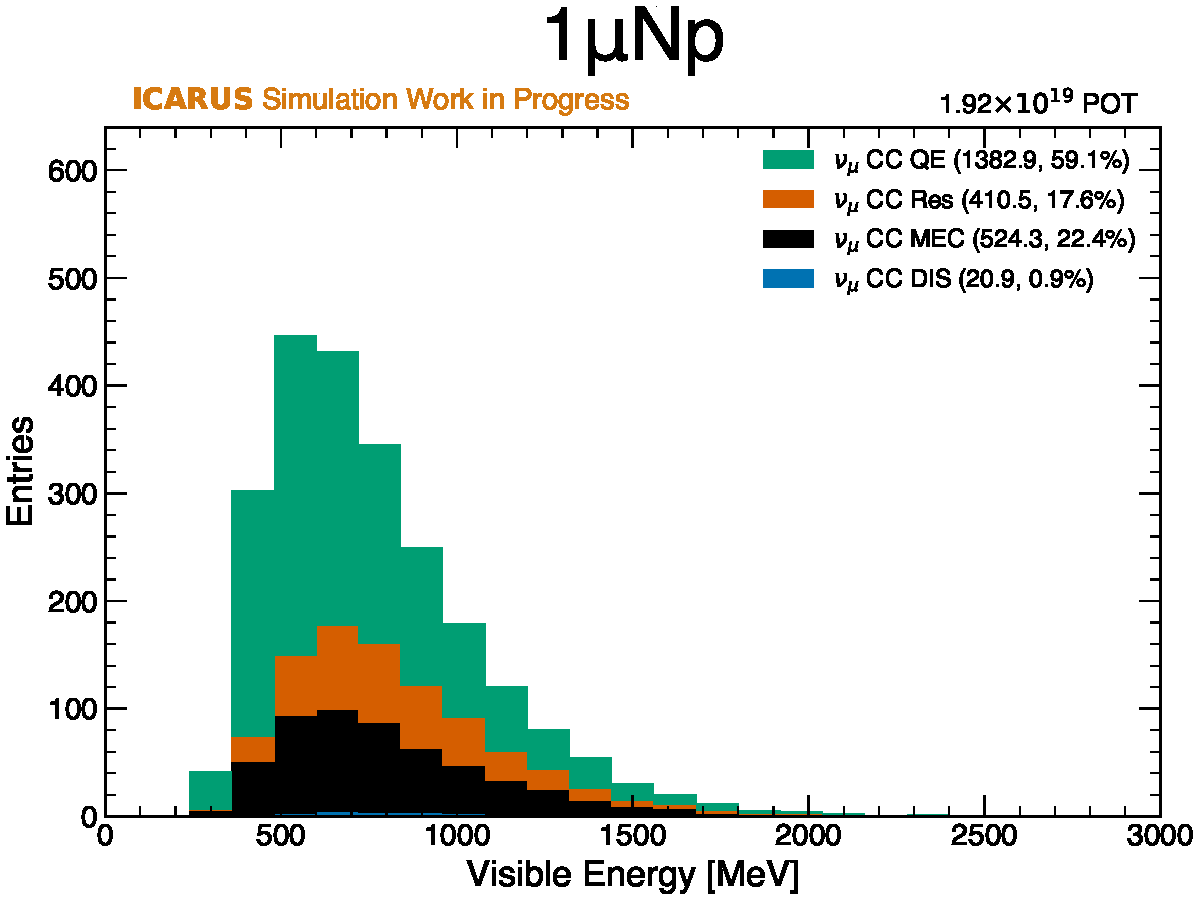
\includegraphics[width=0.48\textwidth]{figures/neutrino_selection/signal_hist1d_1muNp_visible_energy.pdf}\\
    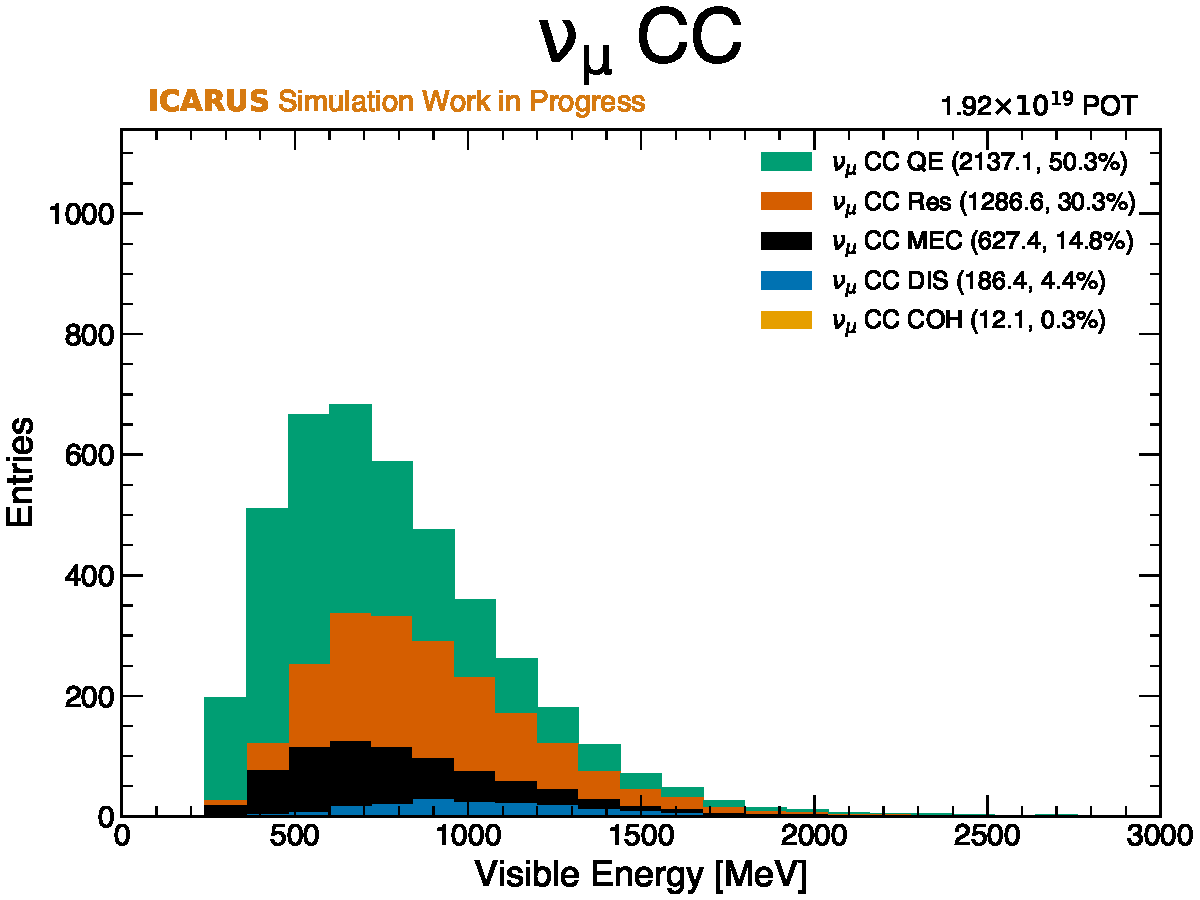
\includegraphics[width=0.48\textwidth]{figures/neutrino_selection/signal_hist1d_1muX_visible_energy.pdf}\\
    \caption{Total visible energy of the interaction for each of the signal channels: from top to bottom $\mathrm{1\mu 1p}$, $\mathrm{1\mu Np}$, and $\nu_\mu$ CC inclusive.}
    \label{fig:visible_energy}
\end{figure}

\paragraph{Muon Transverse Momentum ($\mathbf{p_T^\mu}$):}
The component of muon momentum perpendicular to the neutrino beam direction. This should generally be balanced by the transverse momentum of the hadronic system in the absence of final state interactions, as described in more detail below in the text on kinematic imbalance variables.

\paragraph{Leading Proton Transverse Momentum ($\mathbf{p_T^p}$):}
The component of the momentum of the most energetic primary proton perpendicular to the neutrino beam direction.

\begin{figure}[!htb]
    \centering
    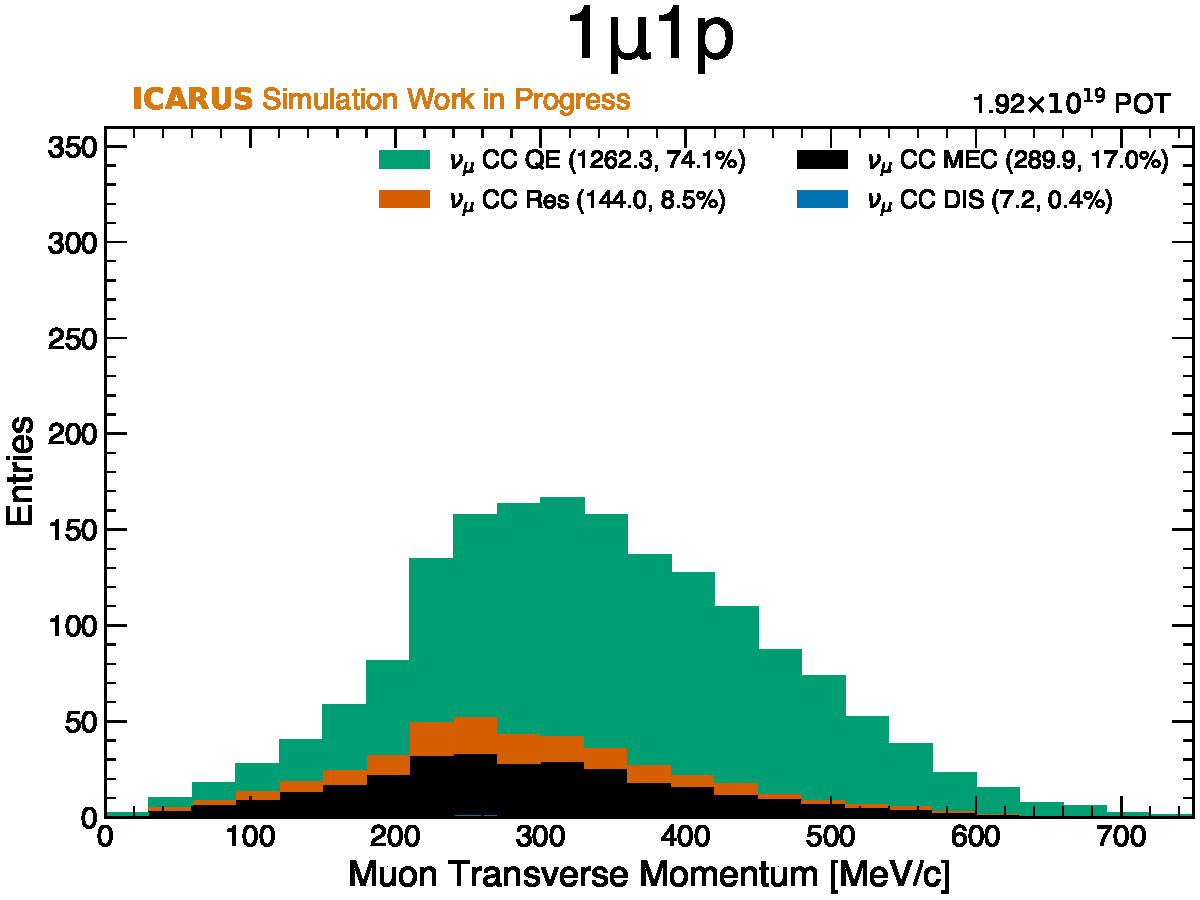
\includegraphics[width=0.48\textwidth]{figures/neutrino_selection/signal_hist1d_1mu1p_muon_pt.pdf}
    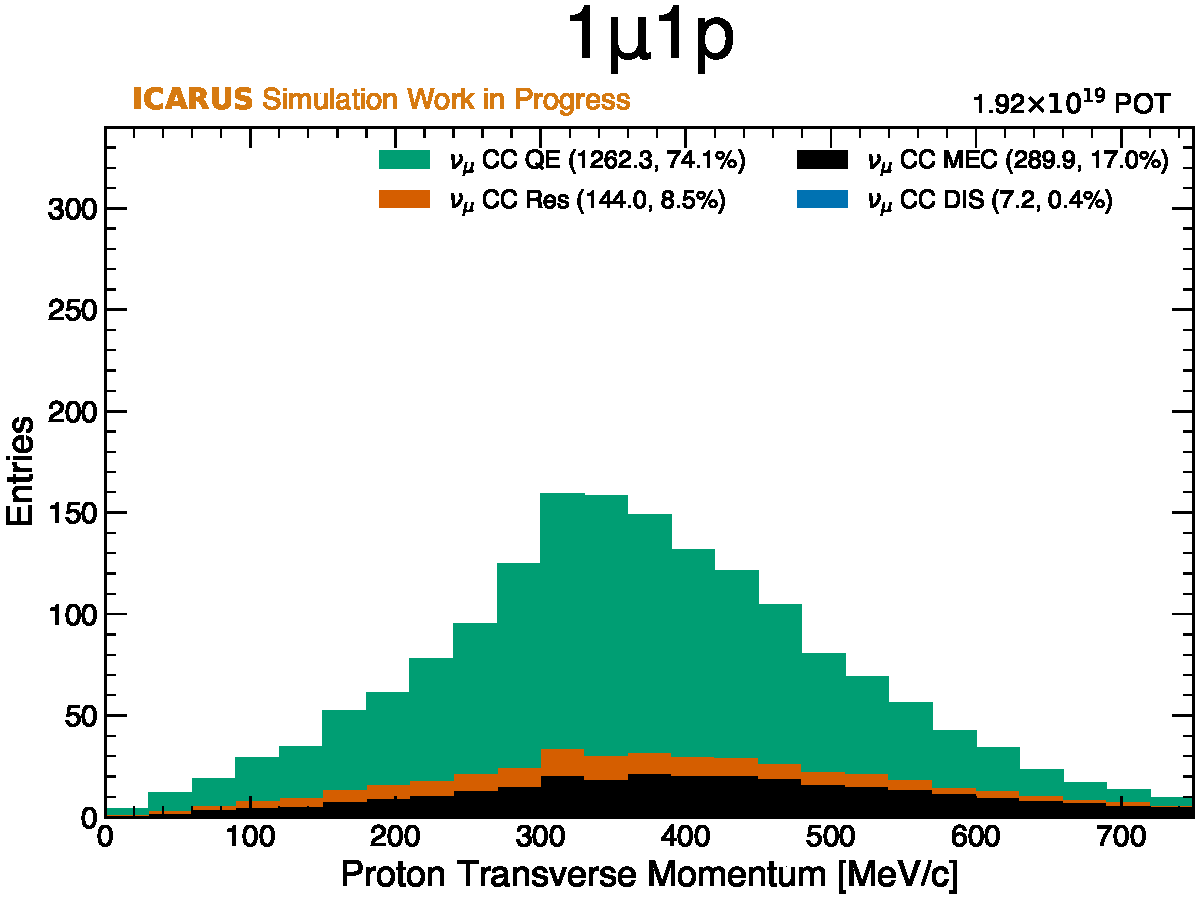
\includegraphics[width=0.48\textwidth]{figures/neutrino_selection/signal_hist1d_1mu1p_proton_pt.pdf}
    \\
    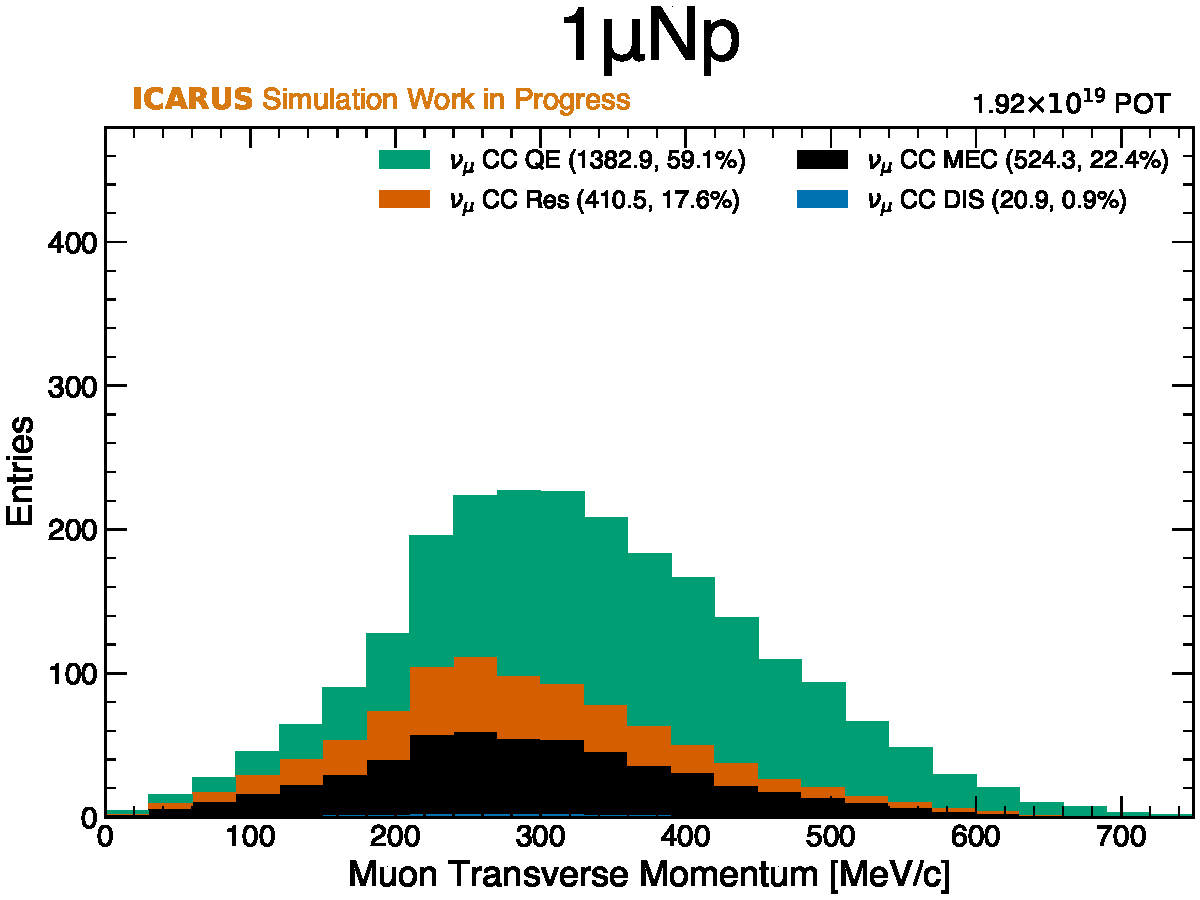
\includegraphics[width=0.48\textwidth]{figures/neutrino_selection/signal_hist1d_1muNp_muon_pt.pdf}
    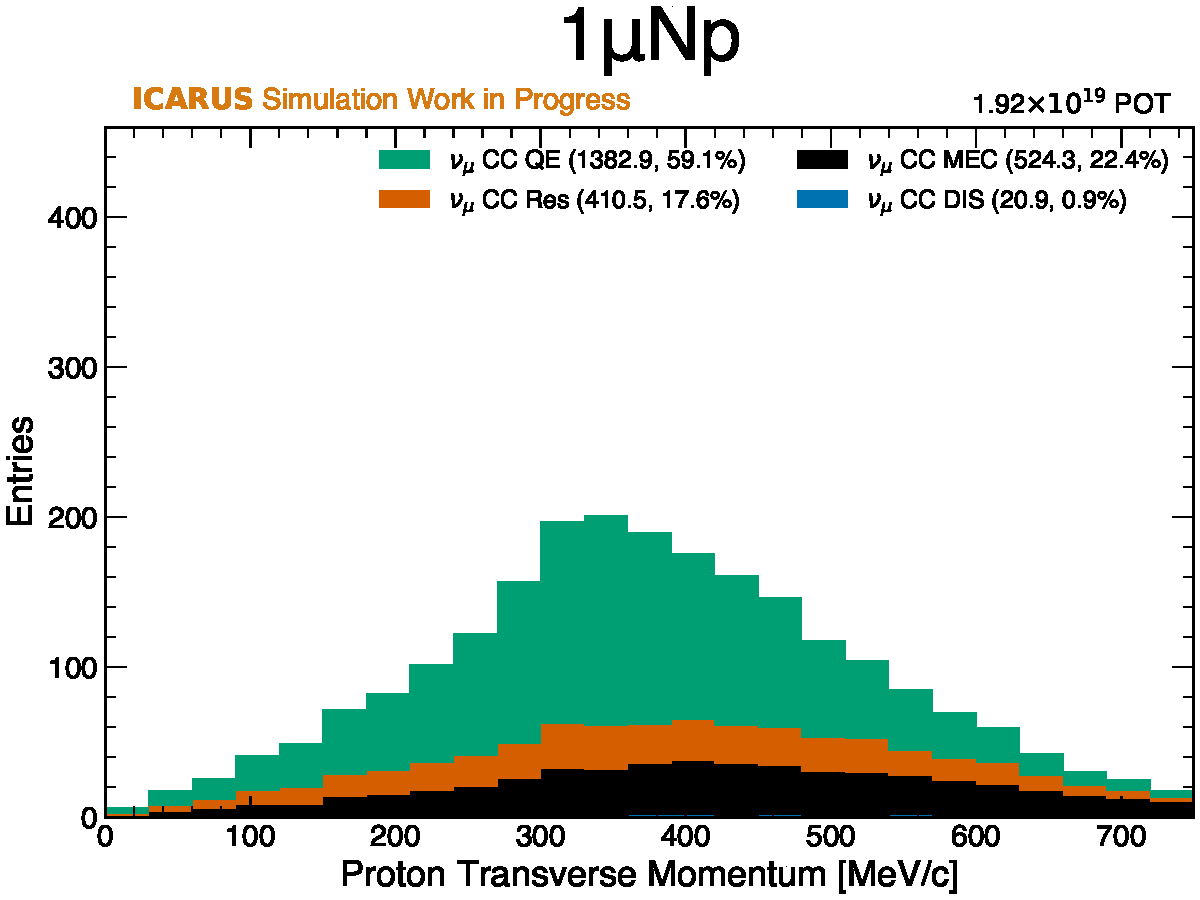
\includegraphics[width=0.48\textwidth]{figures/neutrino_selection/signal_hist1d_1muNp_proton_pt.pdf}
    \\
    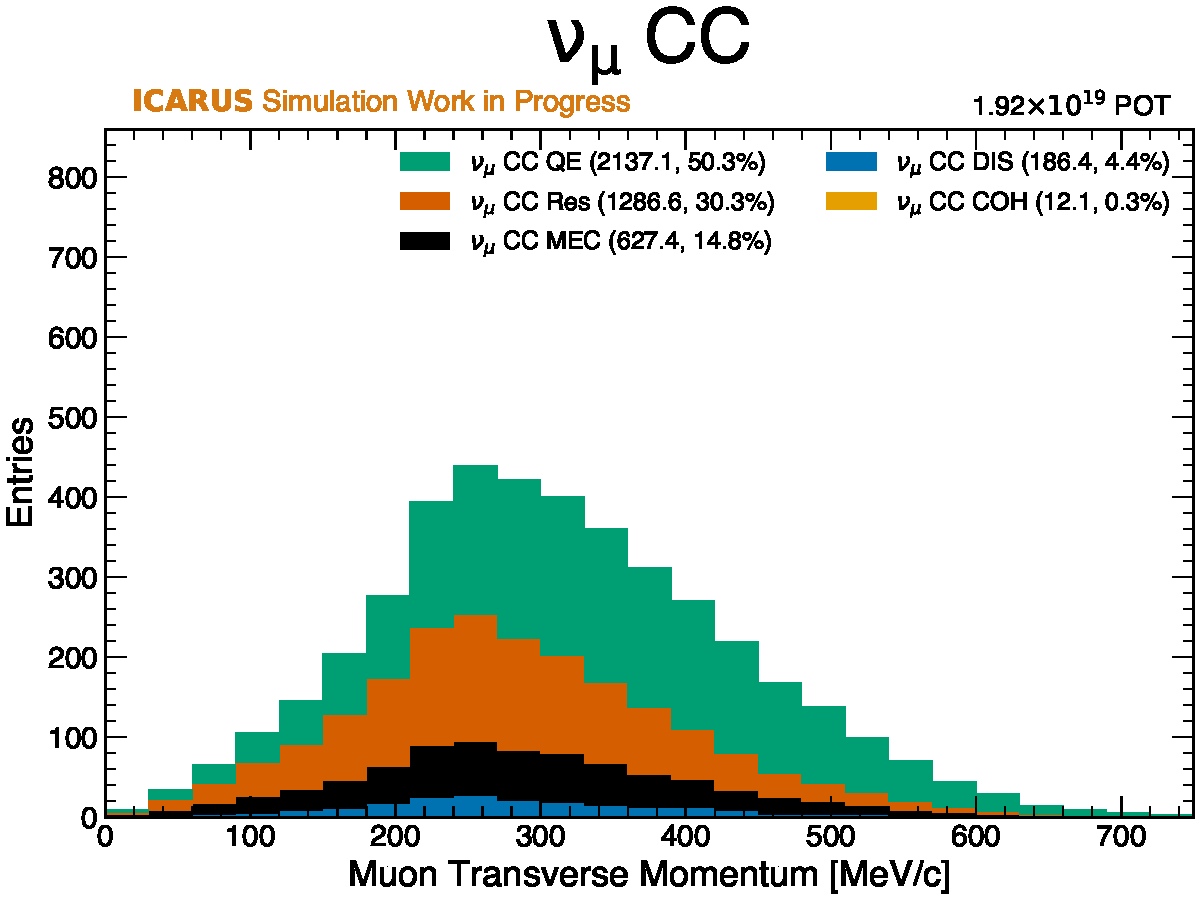
\includegraphics[width=0.48\textwidth]{figures/neutrino_selection/signal_hist1d_1muX_muon_pt.pdf}
    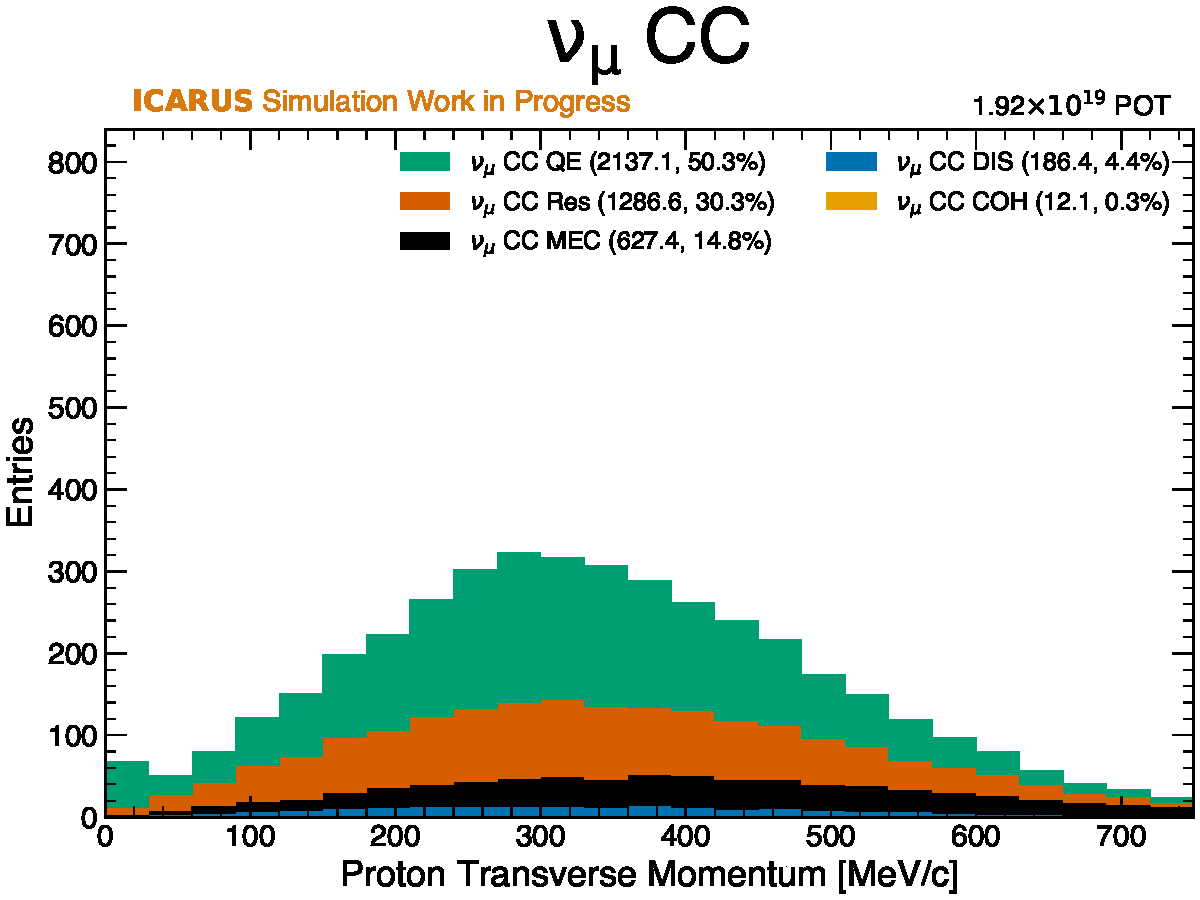
\includegraphics[width=0.48\textwidth]{figures/neutrino_selection/signal_hist1d_1muX_proton_pt.pdf}
    \caption{Transverse momentum of the muon (left) and the most energetic proton (right) for each of the three signal channels: from top to bottom $\mathrm{1\mu 1p}$, $\mathrm{1\mu Np}$, and $\nu_\mu$ CC inclusive.}
    \label{fig:muon_proton_pt}
\end{figure}

\paragraph{Muon Polar Angle ($\mathbf{\theta_\mu}$):}
The polar angle of the muon calculated with respect to the neutrino beam direction (z-axis):
\begin{equation}
    \theta_\mu = \arccos\left(\frac{p^\mu_z}{p^\mu}\right)
\end{equation}

\paragraph{Muon Azimuthal Angle ($\mathbf{\phi_\mu}$):}
The azimuthal angle of the muon calculated with respect to the neutrino beam direction (z-axis):
\begin{equation}
    \phi_\mu = \arccos\left(\frac{p^\mu_x}{p^\mu_T}\right)
\end{equation}

\begin{figure}[!htb]
    \centering
    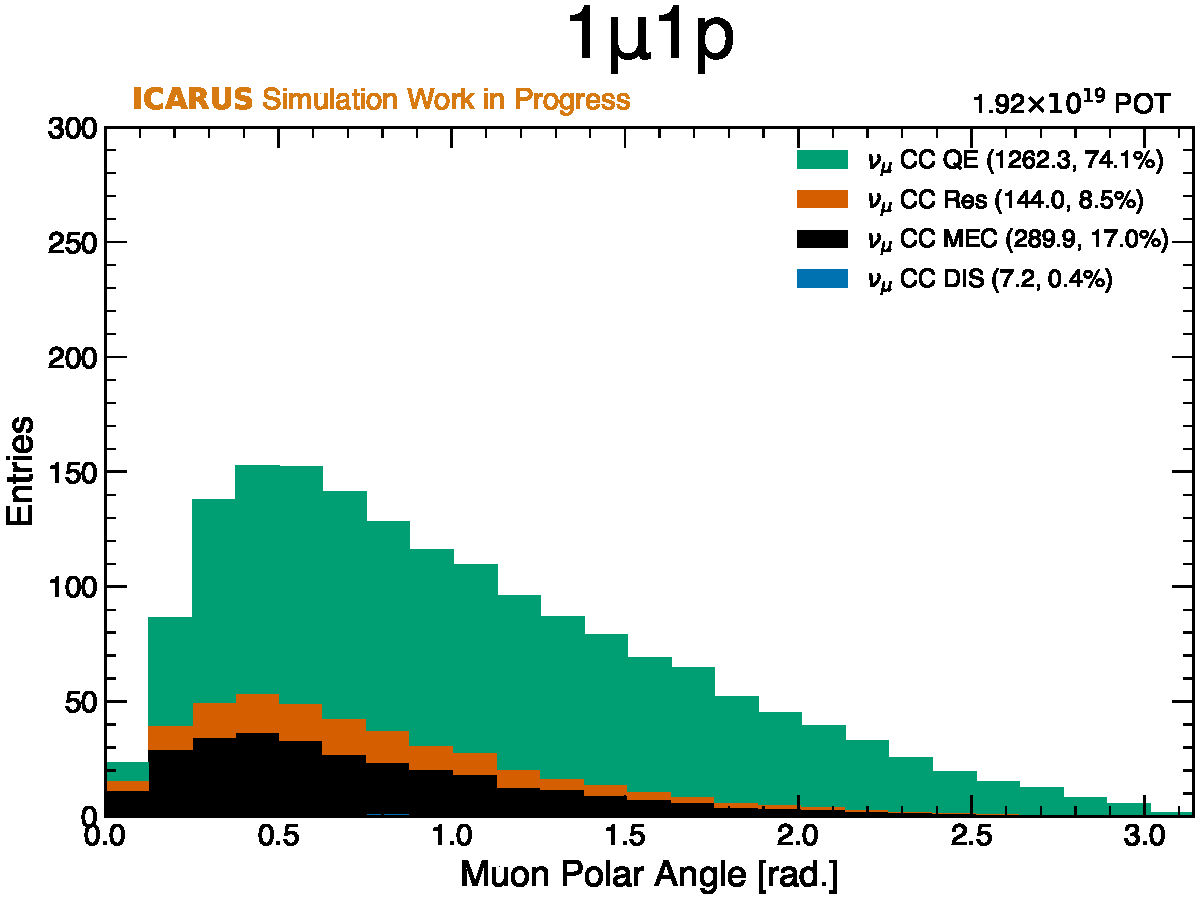
\includegraphics[width=0.48\textwidth]{figures/neutrino_selection/signal_hist1d_1mu1p_muon_polar_angle.pdf}
    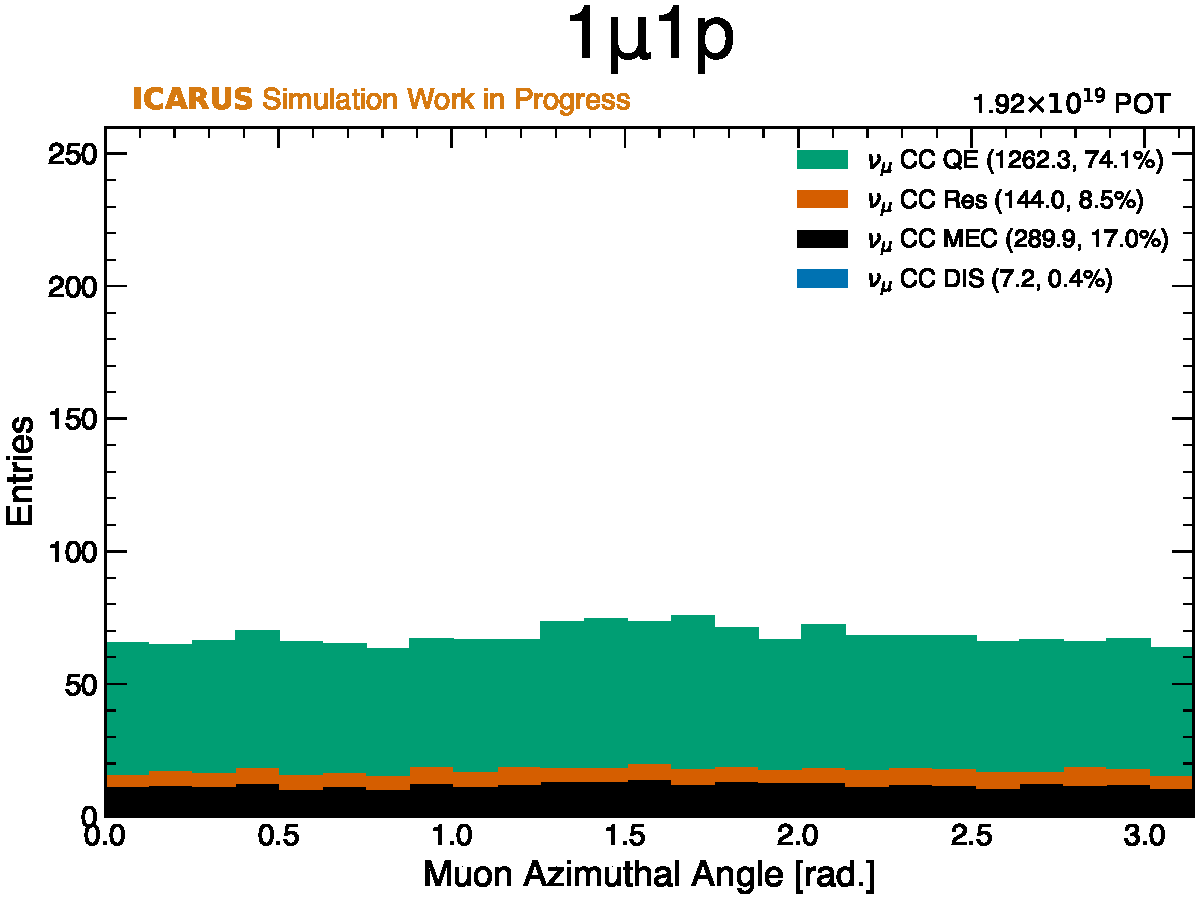
\includegraphics[width=0.48\textwidth]{figures/neutrino_selection/signal_hist1d_1mu1p_muon_azimuthal_angle.pdf}
    \\
    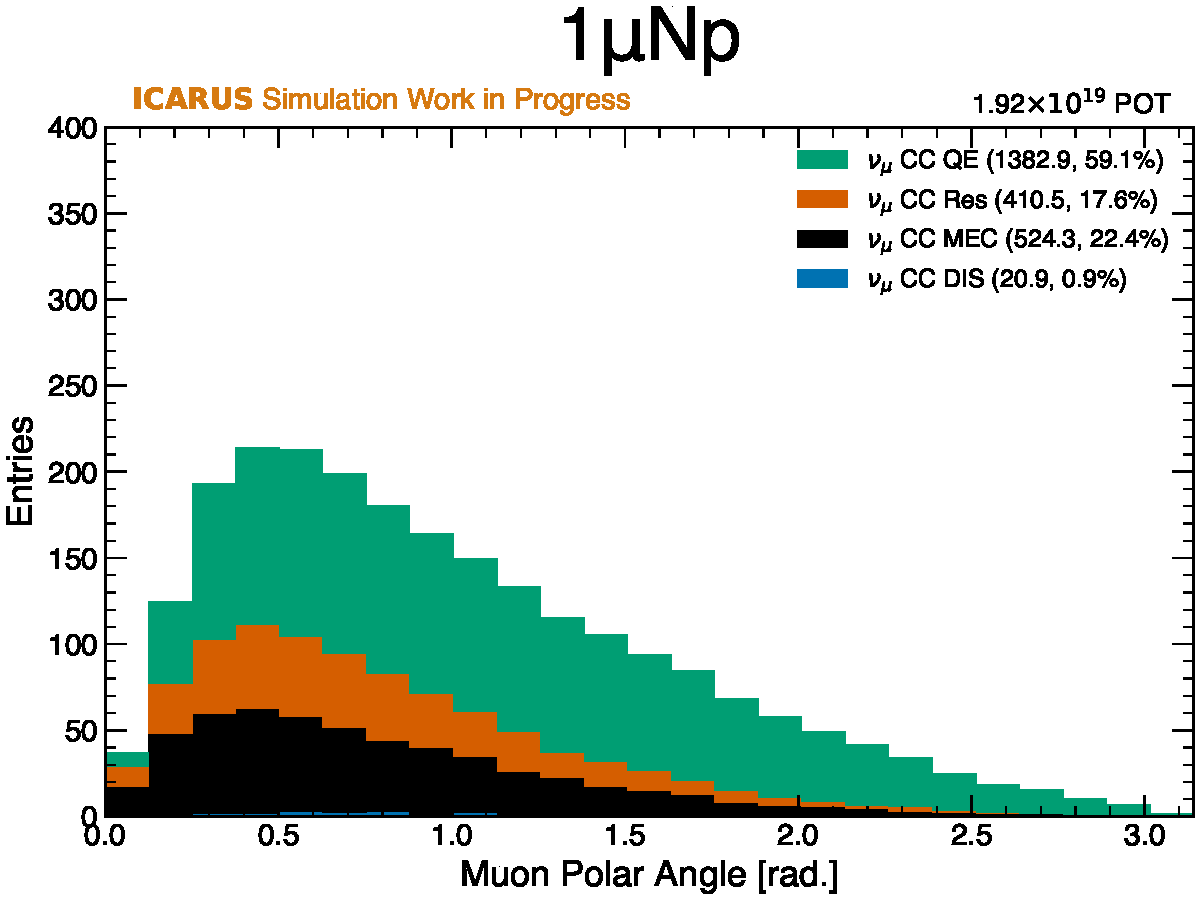
\includegraphics[width=0.48\textwidth]{figures/neutrino_selection/signal_hist1d_1muNp_muon_polar_angle.pdf}
    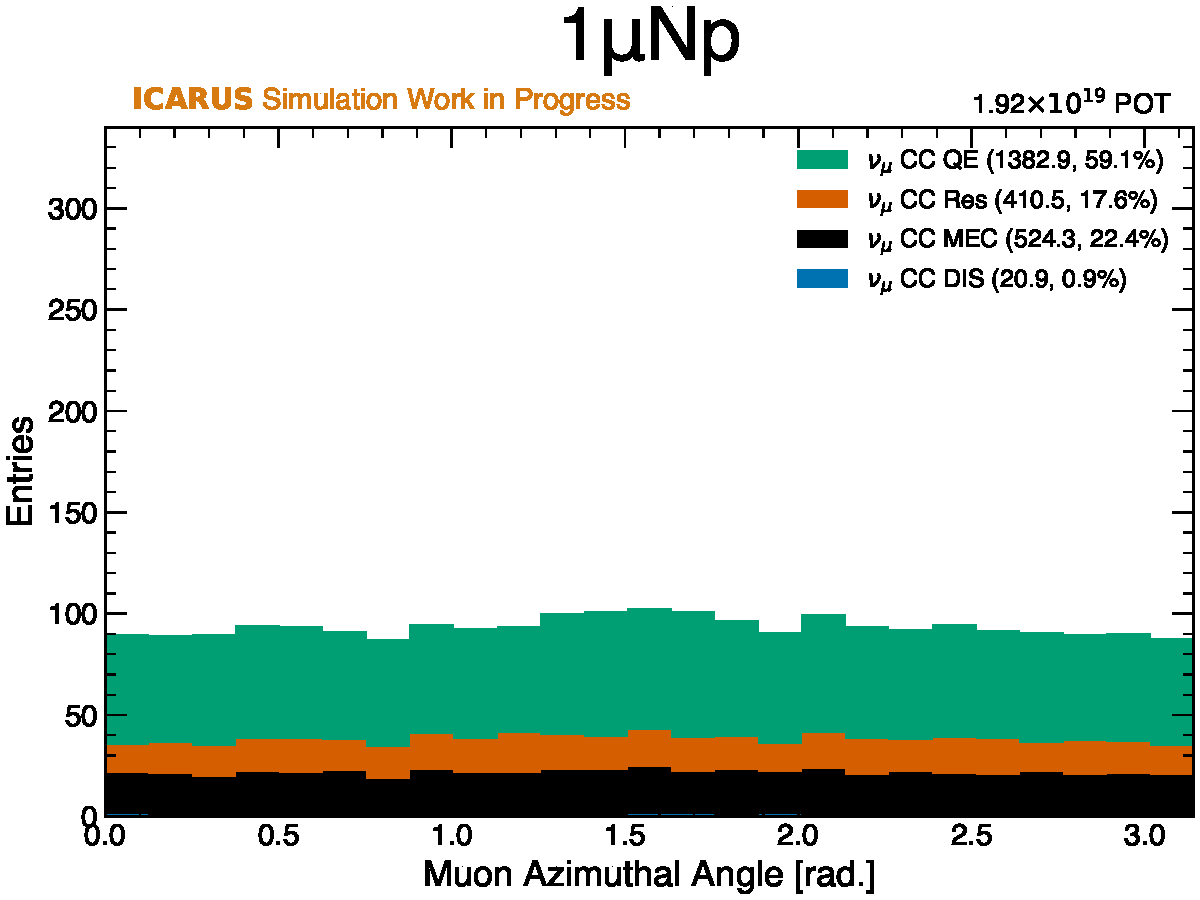
\includegraphics[width=0.48\textwidth]{figures/neutrino_selection/signal_hist1d_1muNp_muon_azimuthal_angle.pdf}
    \\
    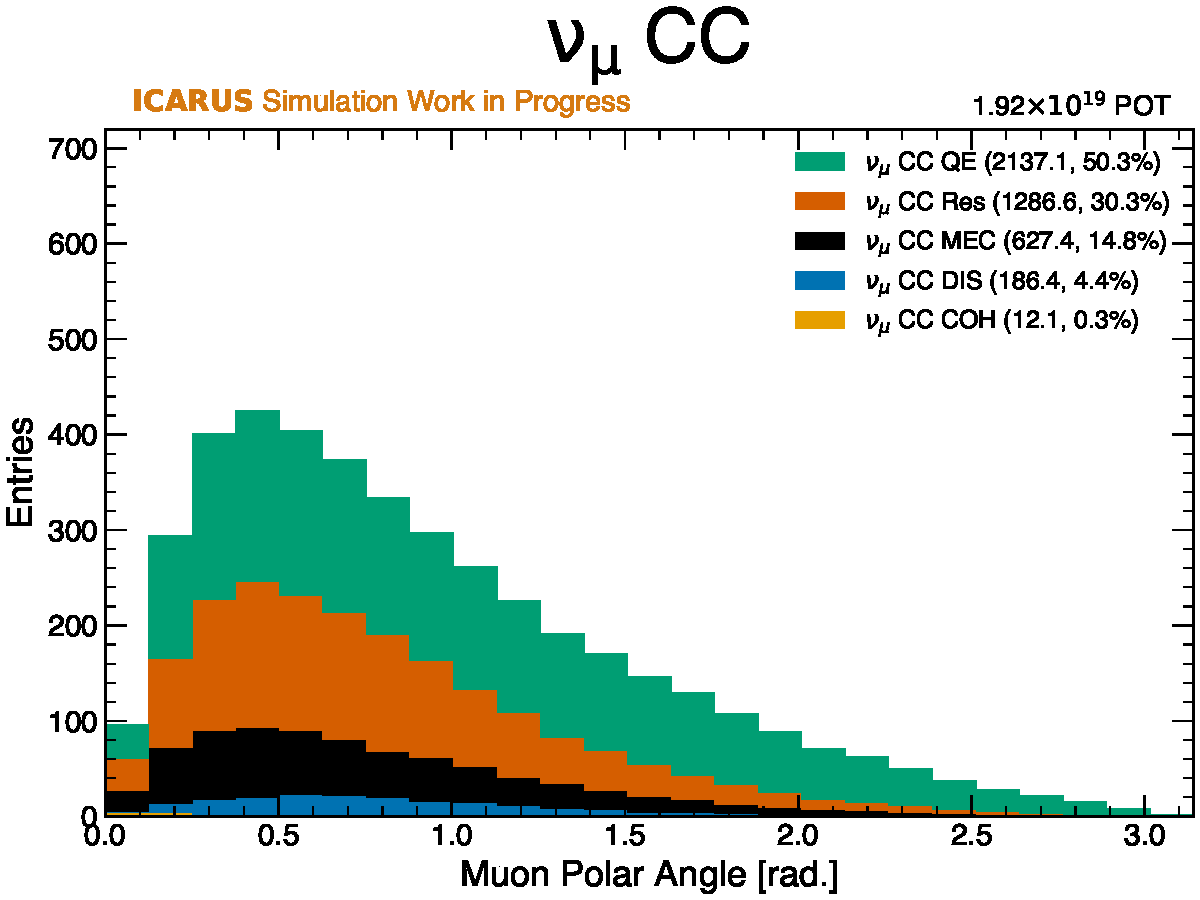
\includegraphics[width=0.48\textwidth]{figures/neutrino_selection/signal_hist1d_1muX_muon_polar_angle.pdf}
    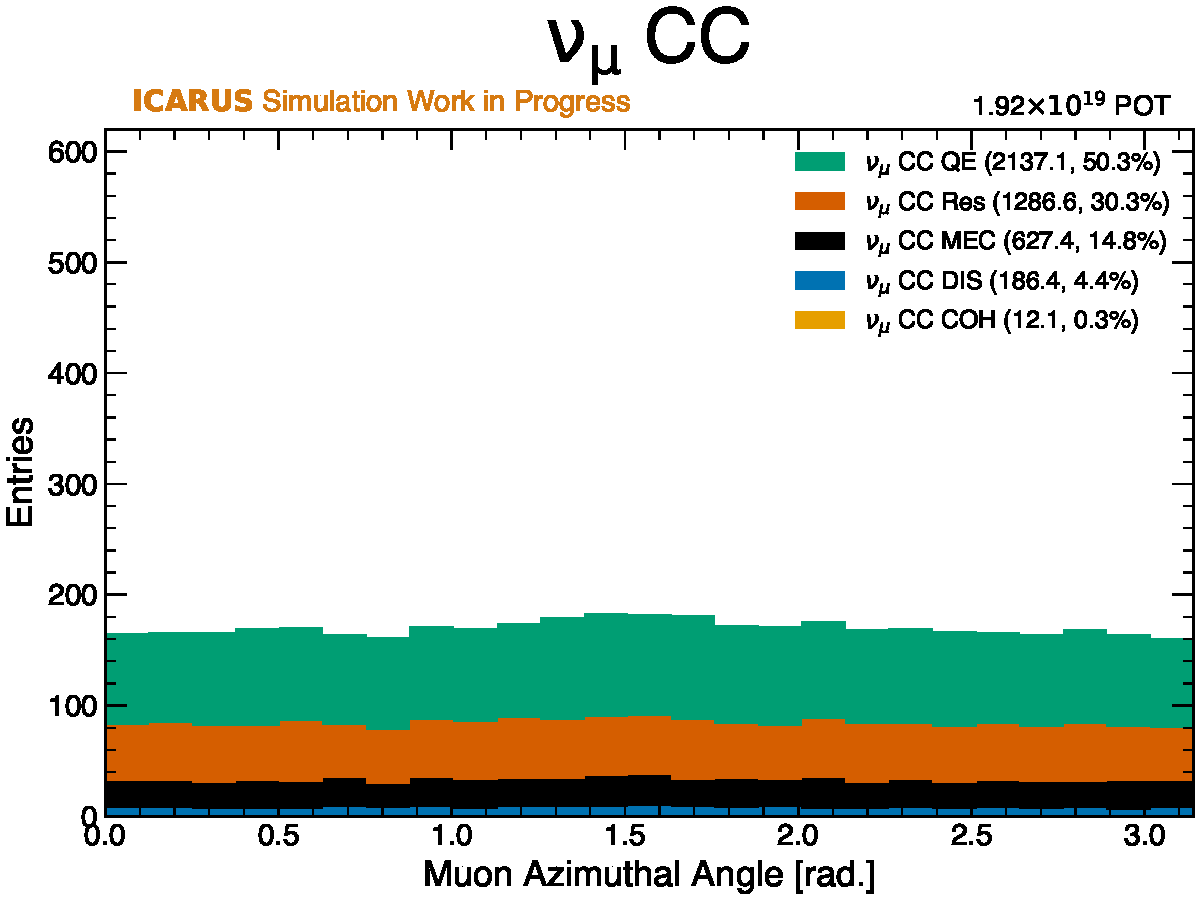
\includegraphics[width=0.48\textwidth]{figures/neutrino_selection/signal_hist1d_1muX_muon_azimuthal_angle.pdf}
    \caption{Polar angle (left) and azimuthal angle (right) of the muon for each of the three signal channels: from top to bottom $\mathrm{1\mu 1p}$, $\mathrm{1\mu Np}$, and $\nu_\mu$ CC inclusive.}
    \label{fig:muon_angles}
\end{figure}

\paragraph{Opening Angle ($\mathbf{\theta_{\mu p}}$):}
The angle between the muon and the leading proton.
\begin{equation}
    \theta_{\mu p} = \arccos\left(\frac{\vec{p\ }^\mu \cdot \vec{p\ }^p}{|\vec{p\ }^\mu||\vec{p\ }^p|}\right)
\end{equation}

\begin{figure}[!htb]
    \centering
    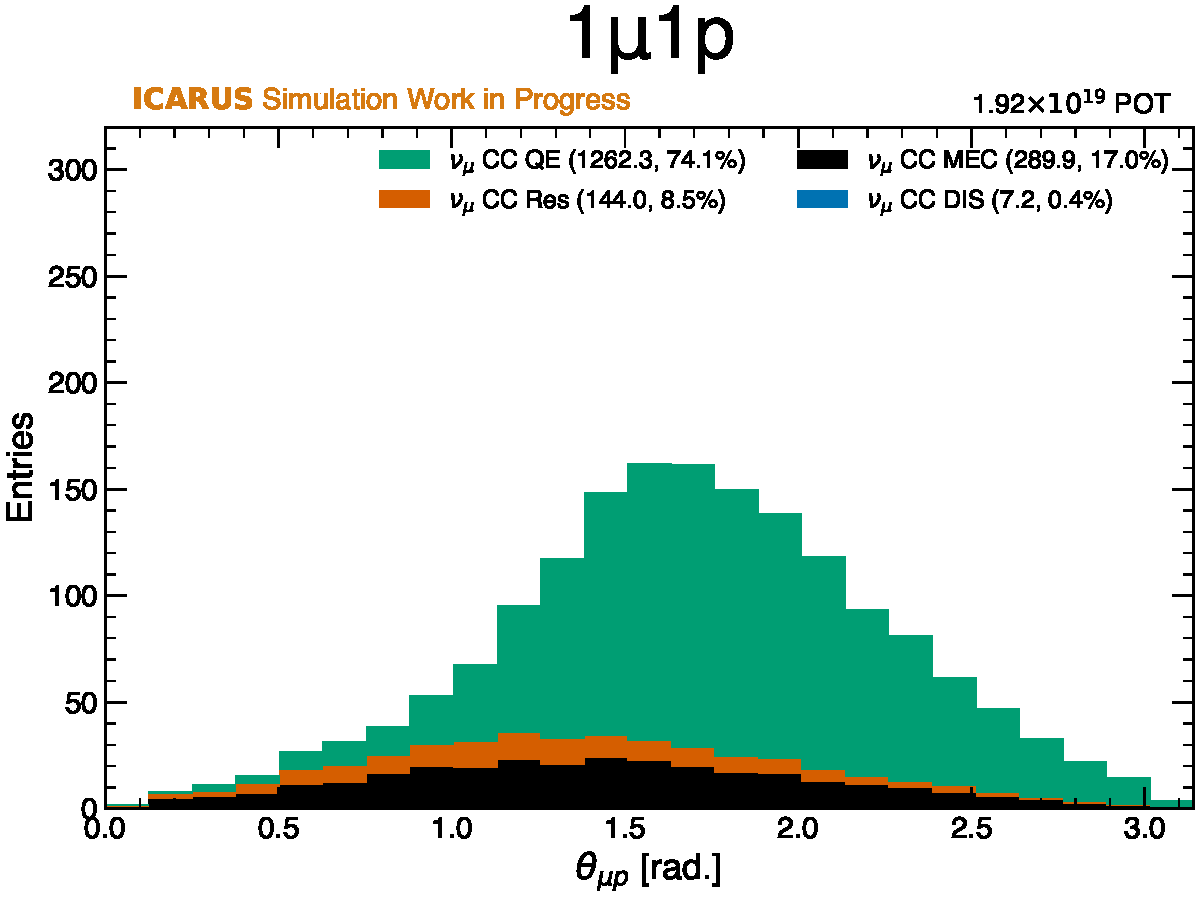
\includegraphics[width=0.48\textwidth]{figures/neutrino_selection/signal_hist1d_1mu1p_opening_angle.pdf}\\
    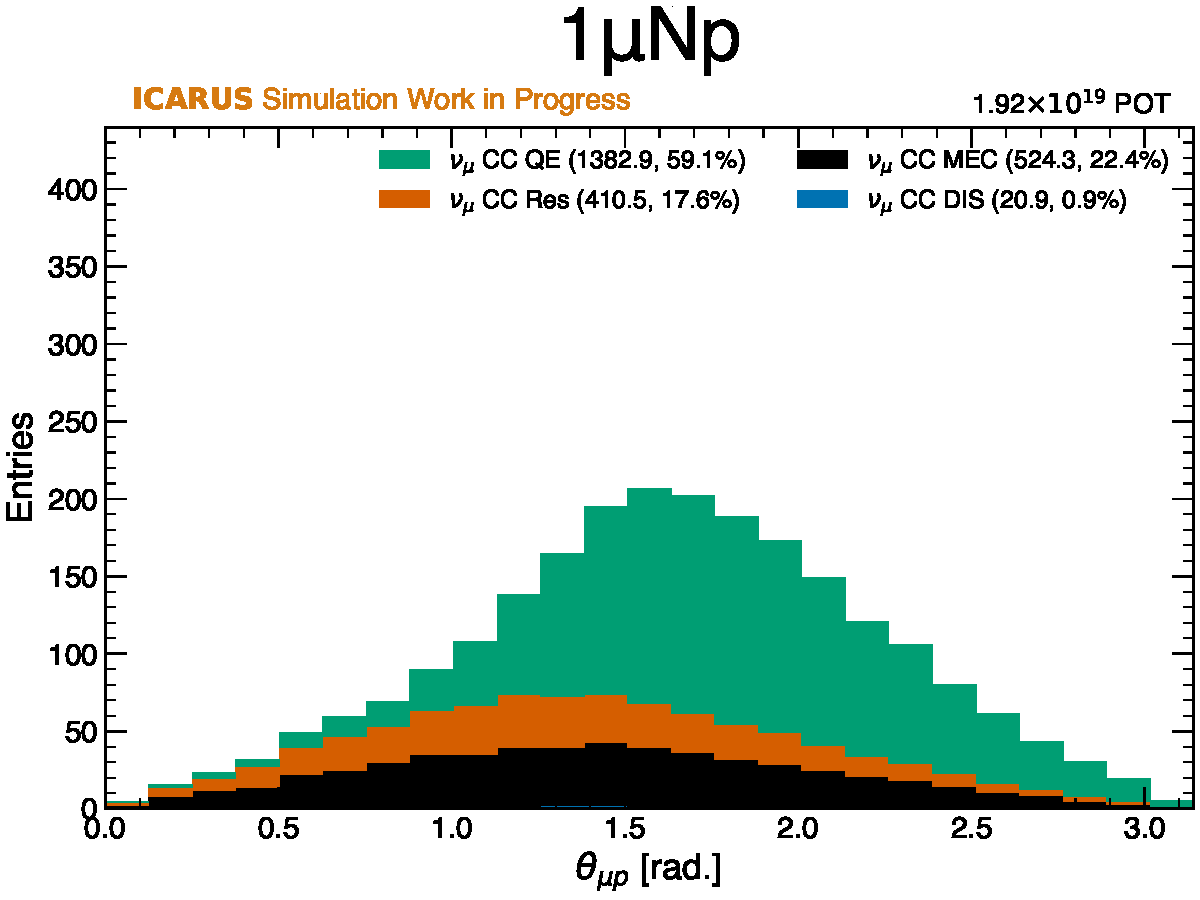
\includegraphics[width=0.48\textwidth]{figures/neutrino_selection/signal_hist1d_1muNp_opening_angle.pdf}\\
    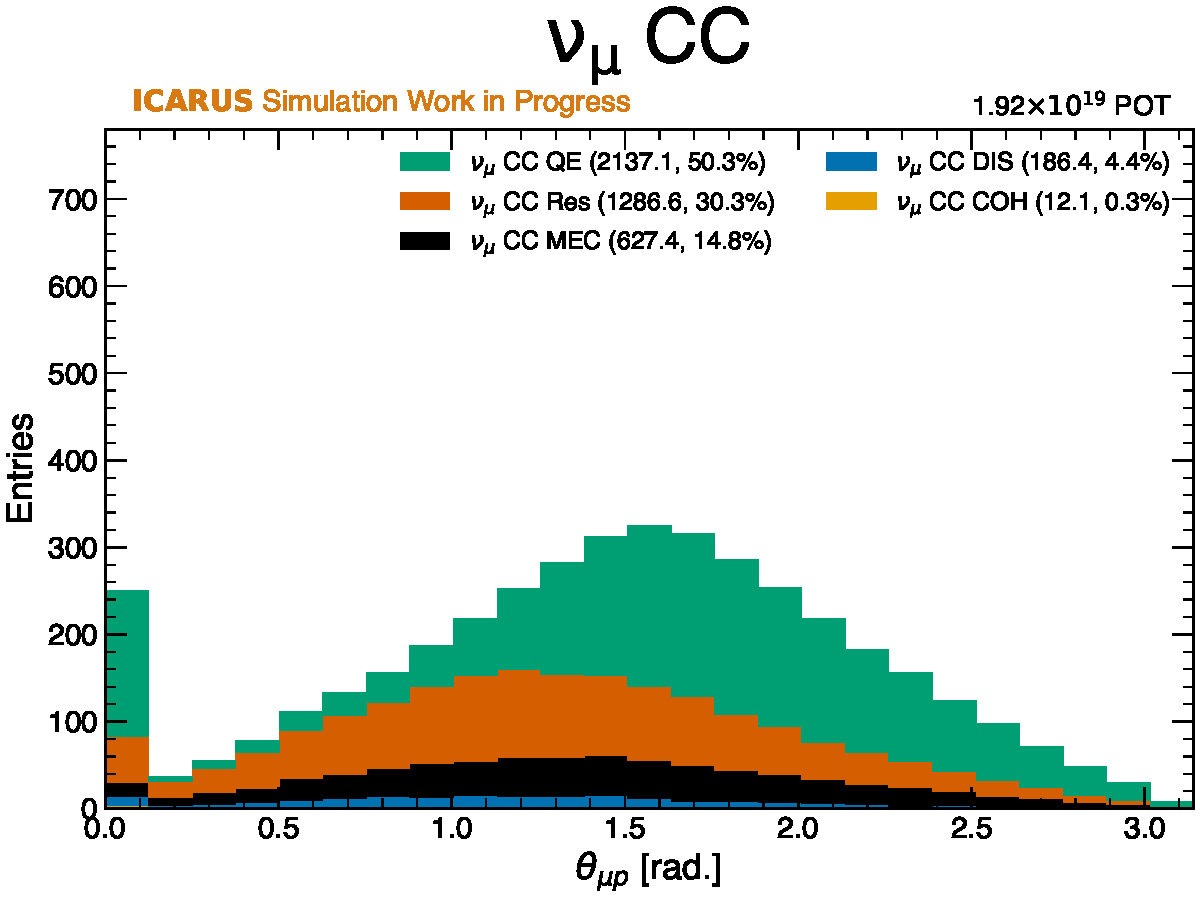
\includegraphics[width=0.48\textwidth]{figures/neutrino_selection/signal_hist1d_1muX_opening_angle.pdf}\\
    \caption{The muon-proton opening angle for each of the three signal channels: from top to bottom $\mathrm{1\mu 1p}$, $\mathrm{1\mu Np}$, and $\nu_\mu$ CC inclusive. The peak at the lowest bin in the inclusive channel is from interactions where no proton is present.}
    \label{fig:opening_angle}
\end{figure}

\subsubsection{Kinematic Imbalance Variables}
\label{sec:kinematic_imbalance_variables}

The axis of the beam defines the direction along which the momentum of the interacting neutrino is oriented. The transverse plane is defined as the plane perpendicular to the neutrino beam direction, while the longitudinal direction is defined as oriented along the neutrino beam direction. From conservation of momentum, the momentum in the transverse plane should sum to zero in the absence of initial state nucleon transverse momentum and final state interactions (FSI). Fermi motion inside the nucleus produces non-zero transverse momentum even for quasi-elastic (QE) interactions. More complex interactions such as resonant pion production and deep inelastic scattering can produce final states similar to QE interactions, but with additional transverse momentum that populates the region above the Fermi momentum. These variables are natural choices for probing the effects of FSI and for measuring neutrino interaction cross sections.

In the ICARUS geometry, the beam axis is defined as the $z$-axis, and the transverse plane is correspondingly the $x$-$y$ plane. For the signal definitions considered in this analysis, there exists a single muon and a combined hadronic system, respectively having momentum $\vec{p\ }^\mu$ and $\vec{p\ }^h$ and transverse components $\vec{p\ }^\mu_T$ and $\vec{p\ }^h_T$. The transverse component of the momentum transfer to the nucleus, $\vec{q}_T$, is defined as equal and opposite to $\vec{p\ }^\mu_T$. Schematically, this is shown in Figure \ref{fig:kinematic_imbalance} within the transverse plane. This formalism, presented in detail in \cite{MicroBooNE2024}, leads to the introduction of several variables:

\begin{figure}
    \centering
    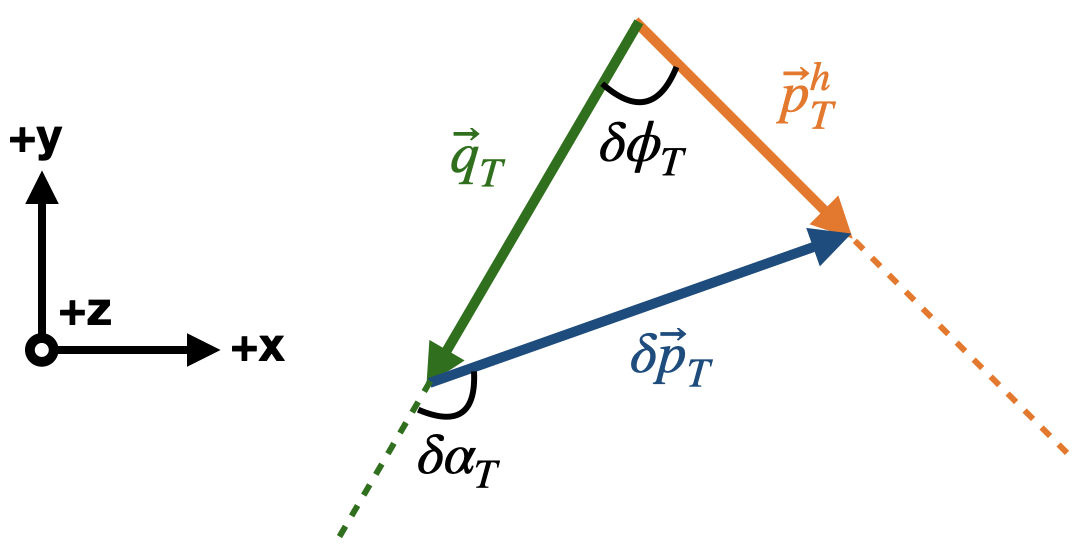
\includegraphics[width=0.5\textwidth]{figures/neutrino_selection/kinematic_imbalance_diagram.png}
    \caption{Diagram showing the each of the chosen kinematic imbalance variables in the transverse plane.}
    \label{fig:kinematic_imbalance}
\end{figure}

\paragraph{$\mathbf{\delta p_T}$:}
The magnitude of the vector difference between the transverse momentum of the muon and the hadronic system. This variable quantifies the amount of transverse momentum that is not accounted for by the reconstructed particles. Large values of this quantity exceeding the Fermi momentum are indicative of FSI.
\begin{equation}
    \delta p_T = \left|\vec{p\ }^\mu_T - \vec{p\ }^h_T\right|
\end{equation}

\begin{figure}[!htb]
    \centering
    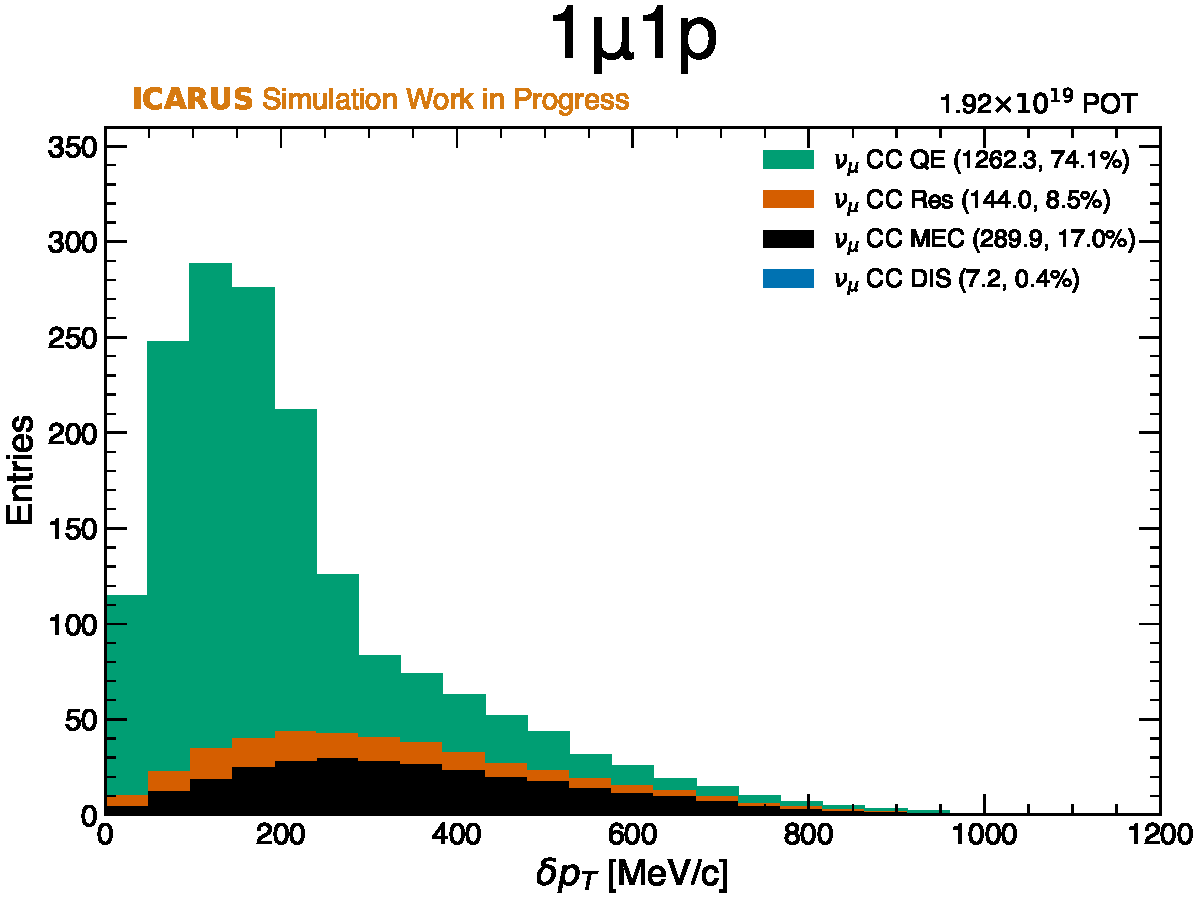
\includegraphics[width=0.48\textwidth]{figures/neutrino_selection/signal_hist1d_1mu1p_delta_pT.pdf}\\
    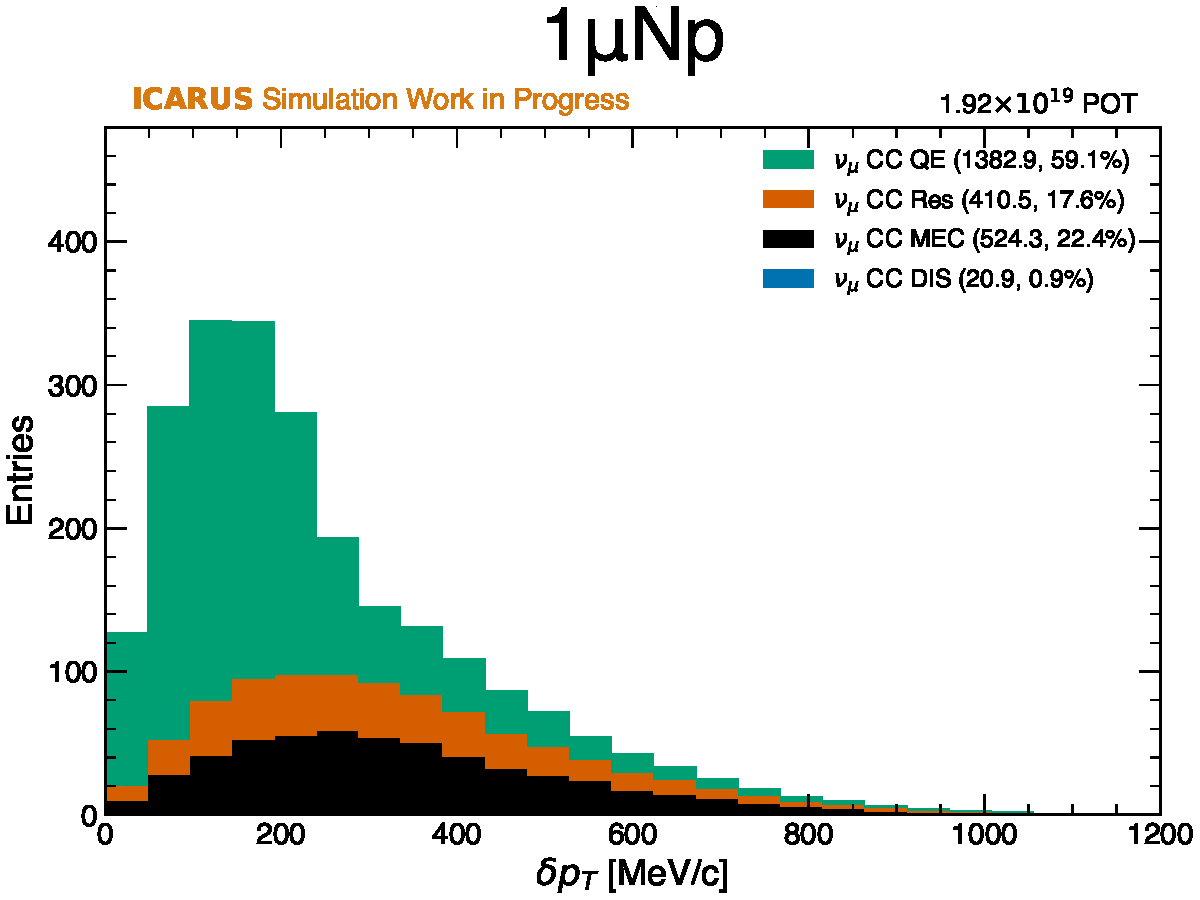
\includegraphics[width=0.48\textwidth]{figures/neutrino_selection/signal_hist1d_1muNp_delta_pT.pdf}\\
    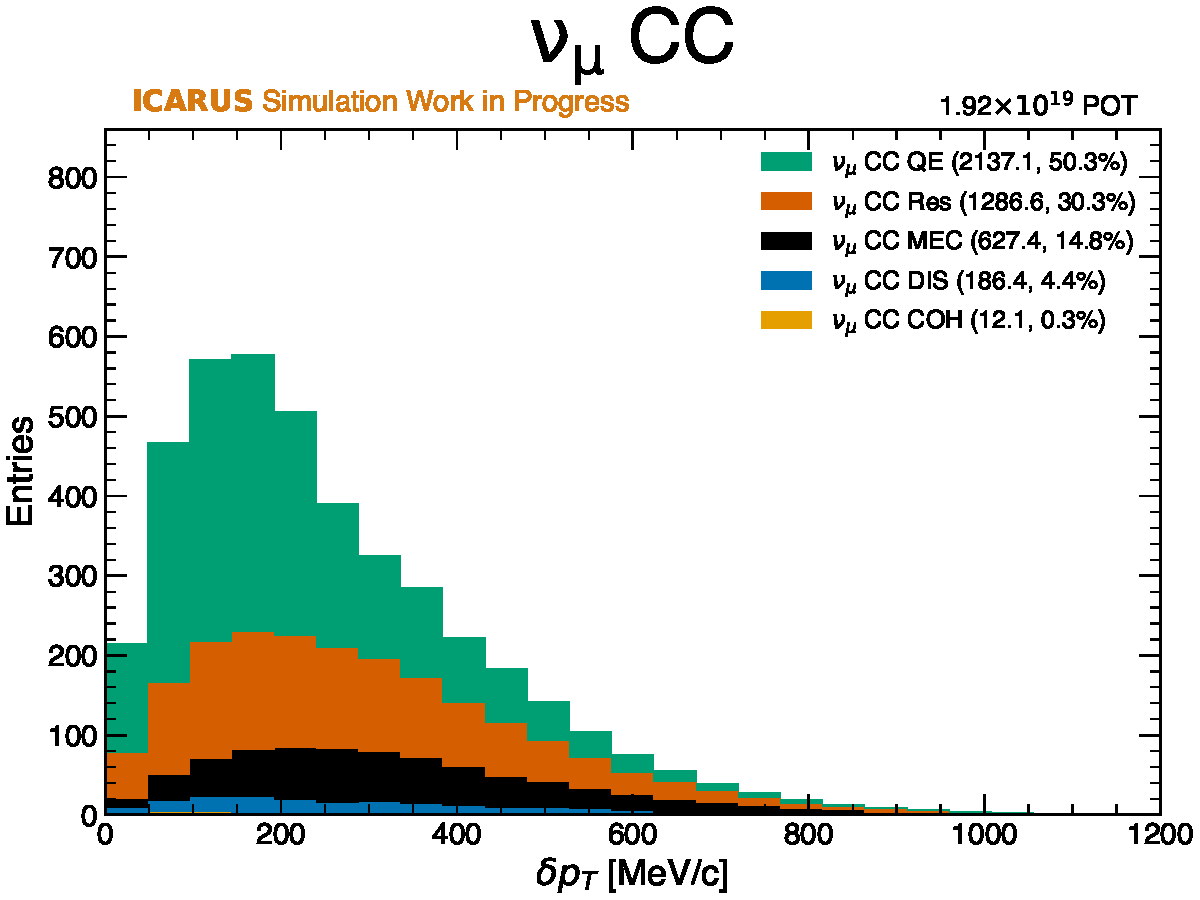
\includegraphics[width=0.48\textwidth]{figures/neutrino_selection/signal_hist1d_1muX_delta_pT.pdf}\\
    \caption{Transverse momentum of the interaction for each of the three signal channels: from top to bottom $\mathrm{1\mu 1p}$, $\mathrm{1\mu Np}$, and $\nu_\mu$ CC inclusive.}
    \label{fig:delta_pT}
\end{figure}

\paragraph{$\mathbf{\delta \phi_T}$:}
The angle between the the transverse momentum transfer vector and the transverse momentum of the hadronic system. In the case of a free and stationary nucleon target, this angle would be zero. Initial state motion leads to small values of this quantity, while FSI can lead to larger values.
\begin{equation}
    \delta \phi_T = \arccos\left(\frac{\vec{p\ }^h_T \cdot \vec{q}_T}{|\vec{p\ }^h_T||\vec{q}_T|}\right)
\end{equation}

\paragraph{$\mathbf{\delta \alpha_T}$:}
The angle between the transverse momentum transfer vector and transverse missing momentum vector. This angle is less sensitive to the initial state motion of the nucleons, but is sensitive to FSI. In the absence of FSI, this quantity does not have a preferred orientation.
\begin{equation}
    \delta \alpha_T = \arccos\left(\frac{\vec{q}_T \cdot \delta \vec{p\ }_T}{|\vec{q}_T||\delta \vec{p\ }_T|}\right)
\end{equation}

\begin{figure}[!htb]
    \centering
    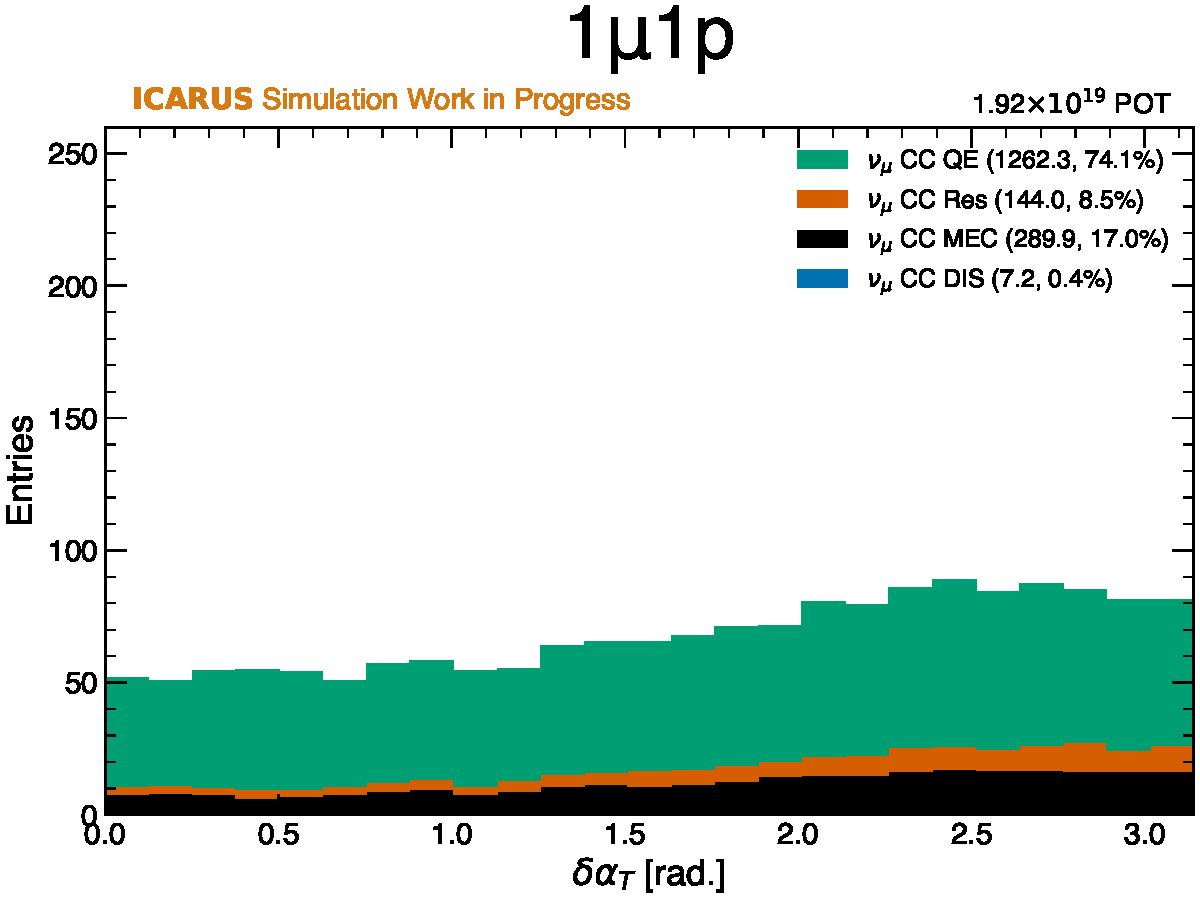
\includegraphics[width=0.48\textwidth]{figures/neutrino_selection/signal_hist1d_1mu1p_delta_alphaT.pdf}
    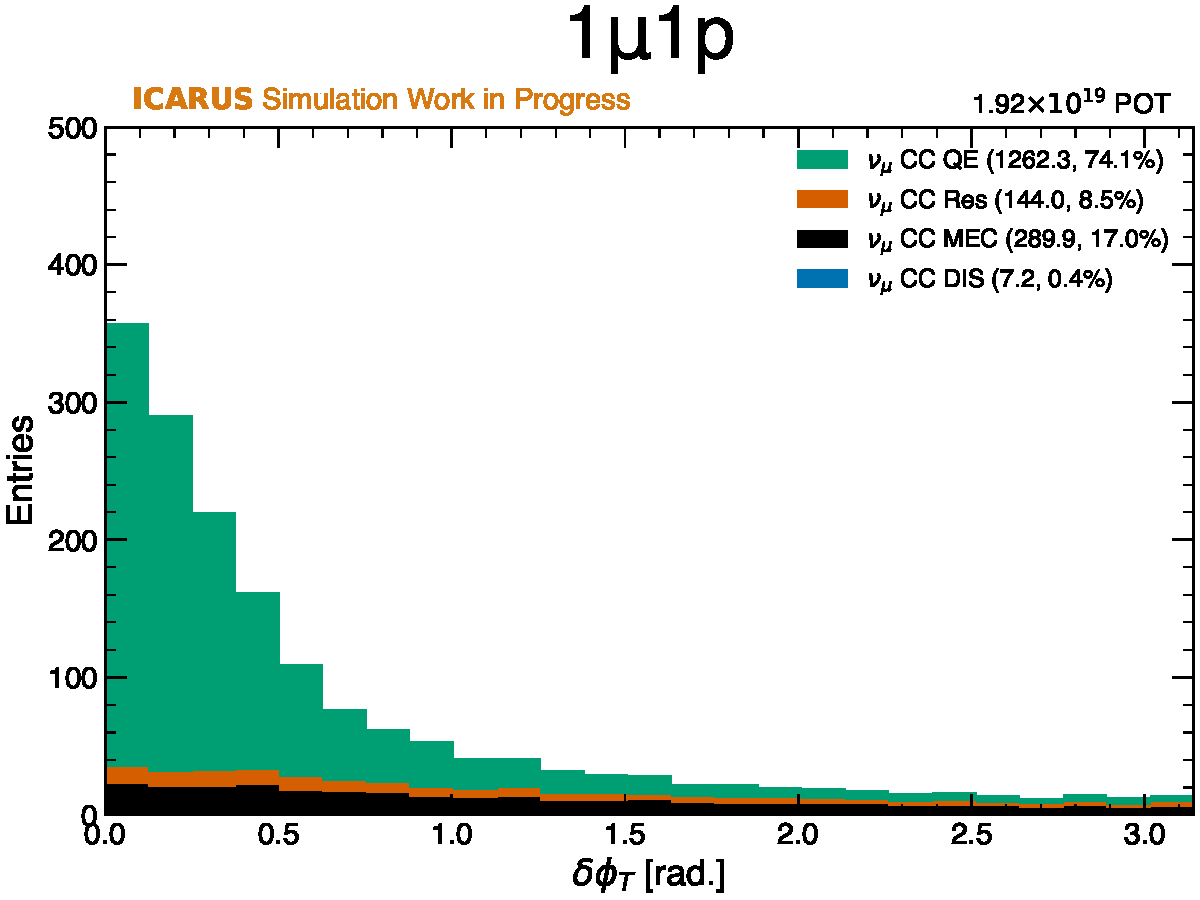
\includegraphics[width=0.48\textwidth]{figures/neutrino_selection/signal_hist1d_1mu1p_delta_phiT.pdf}
    \\
    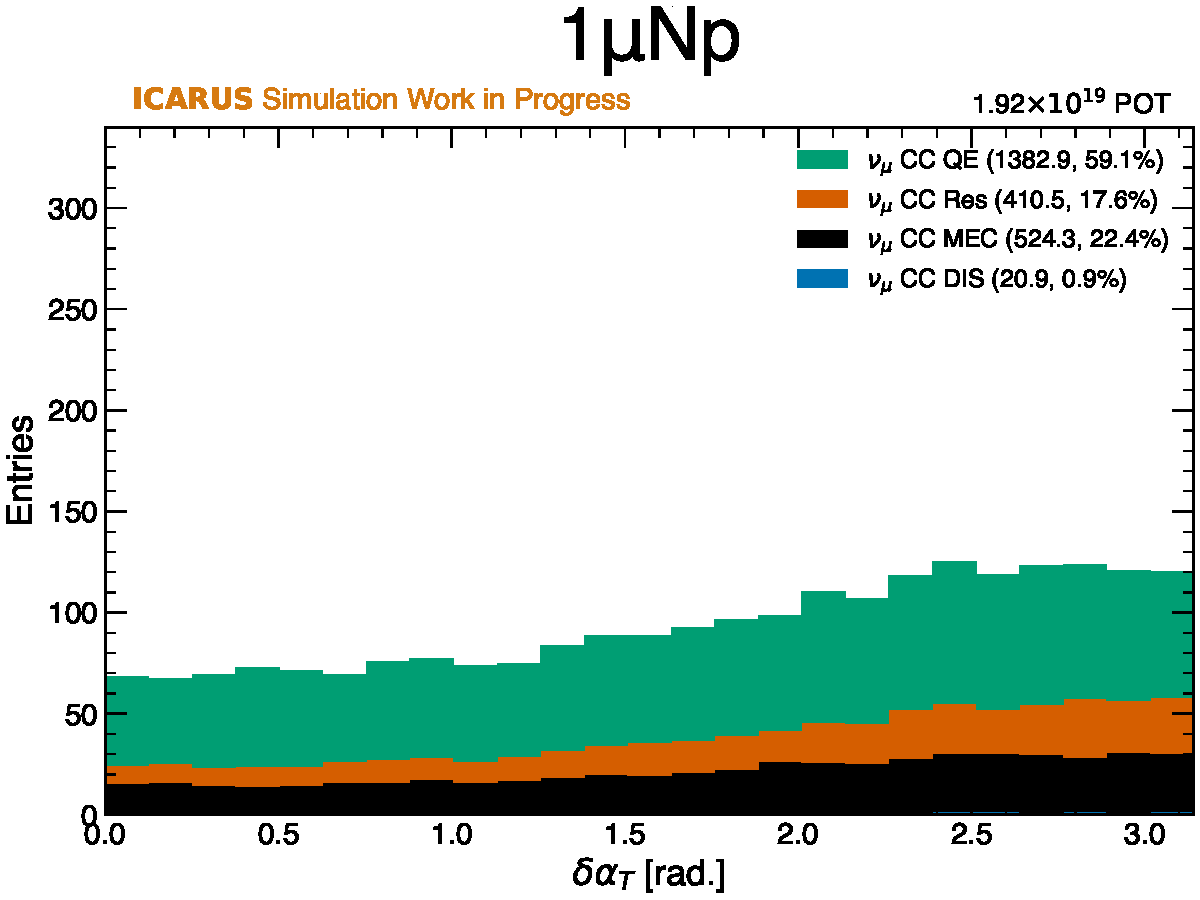
\includegraphics[width=0.48\textwidth]{figures/neutrino_selection/signal_hist1d_1muNp_delta_alphaT.pdf}
    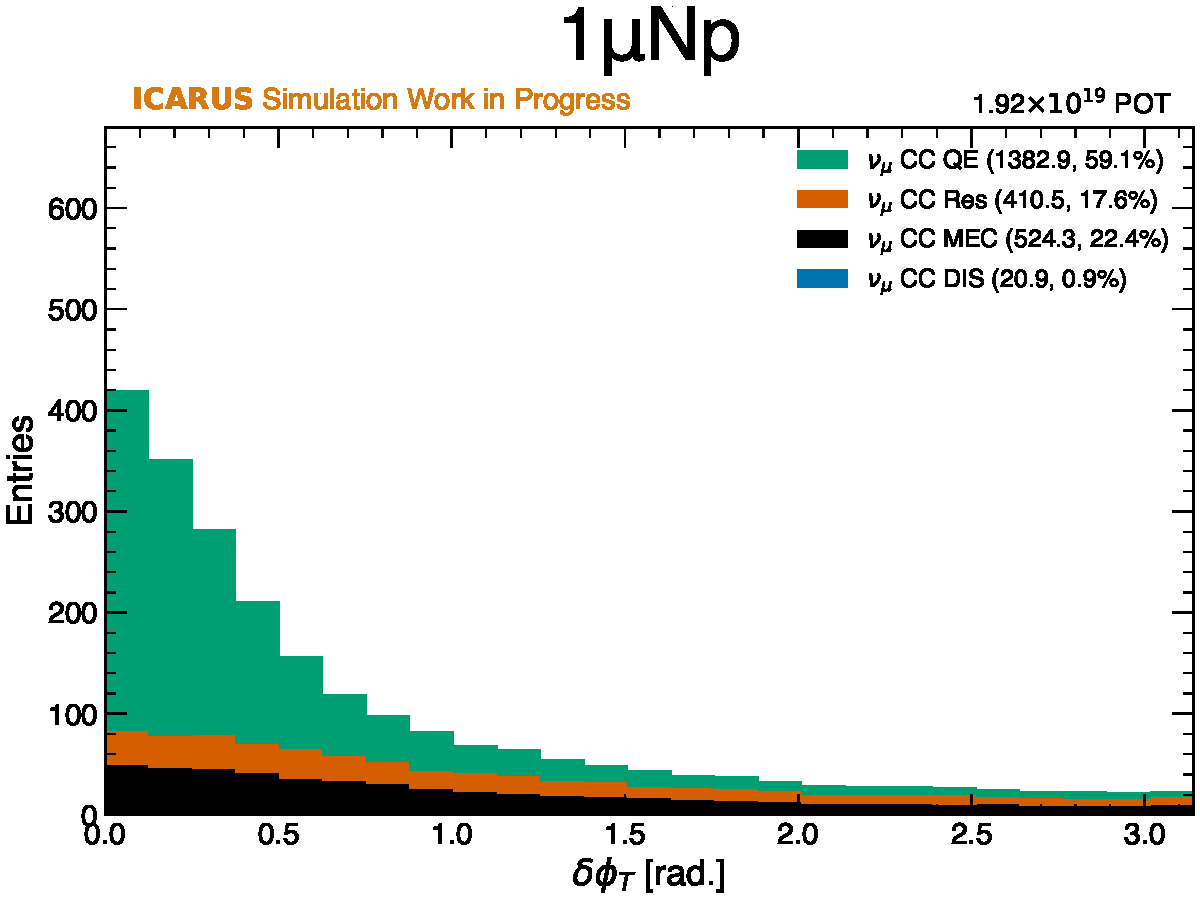
\includegraphics[width=0.48\textwidth]{figures/neutrino_selection/signal_hist1d_1muNp_delta_phiT.pdf}
    \\
    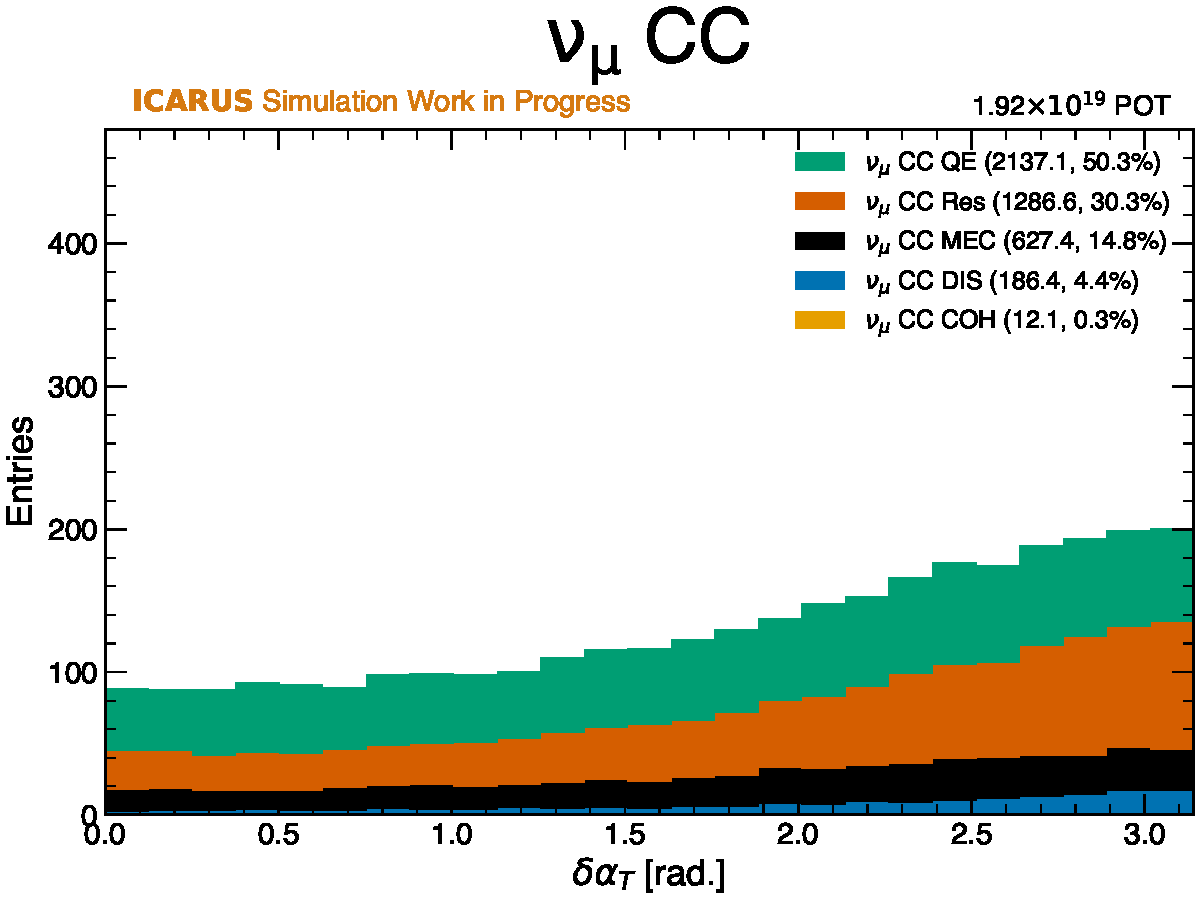
\includegraphics[width=0.48\textwidth]{figures/neutrino_selection/signal_hist1d_1muX_delta_alphaT.pdf}
    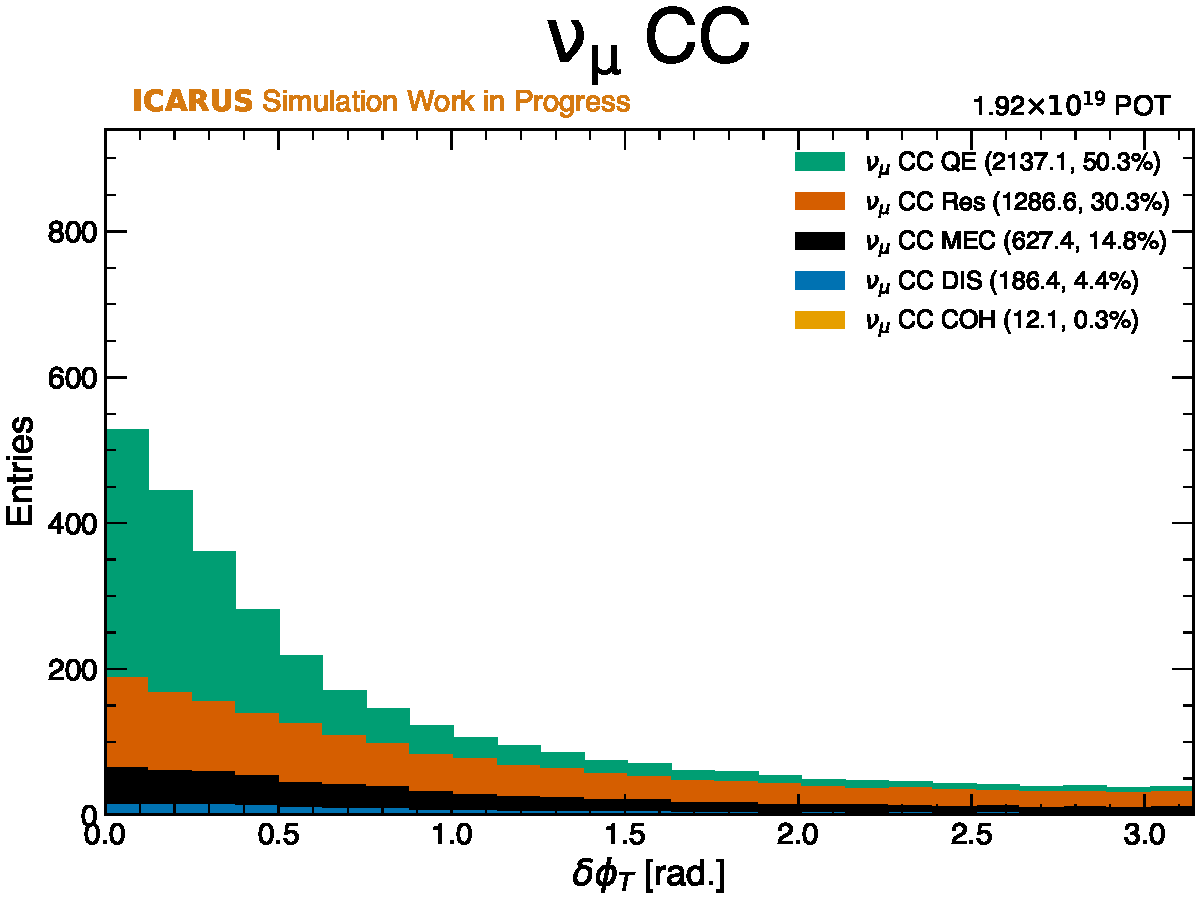
\includegraphics[width=0.48\textwidth]{figures/neutrino_selection/signal_hist1d_1muX_delta_phiT.pdf}
    \caption{Kinematic imbalance variables $\delta \alpha_T$ (left) and $\delta \phi_T$ (right) for each of the three signal channels: from top to bottom $\mathrm{1\mu 1p}$, $\mathrm{1\mu Np}$, and $\nu_\mu$ CC inclusive.}
    \label{fig:kinematic_imbalance_angles}
\end{figure}

\subsubsection{PID Variables}
\label{sec:pid_variables}

Each particle is assigned scores by a GNN, as described in Section \ref{sec:ml_full_chain}, that provide an indication of how likely the particle is to be a muon, proton, or pion for tracks, or an electron or photon for showers. The PID scores are used to assign a particle type to each reconstructed particle. A difference in the distribution of these scores between data and simulation may indicate a bias in the simulation with respect to data, so it is important to validate that these distributions are in agreement with data.

\paragraph{Muon ``Softmax'' PID Score:}
The muon score assigned to the primary muon of the interaction by the reconstruction. A high score near 1 indicates that the particle is likely to be a muon, while a low score near 0 indicates that the particle is not likely to be a muon.

\paragraph{Proton ``Softmax'' PID Score:}
The proton score assigned to the leading proton of the interaction by the reconstruction. A high score near 1 indicates that the particle is likely to be a proton, while a low score near 0 indicates that the particle is not likely to be a proton. This variable is significantly more peaked than the muon score, presumably because the muon and pion are more similar in terms of their energy deposition and track length, so the range of the plot has been restricted.

\begin{figure}[!htb]
    \centering
    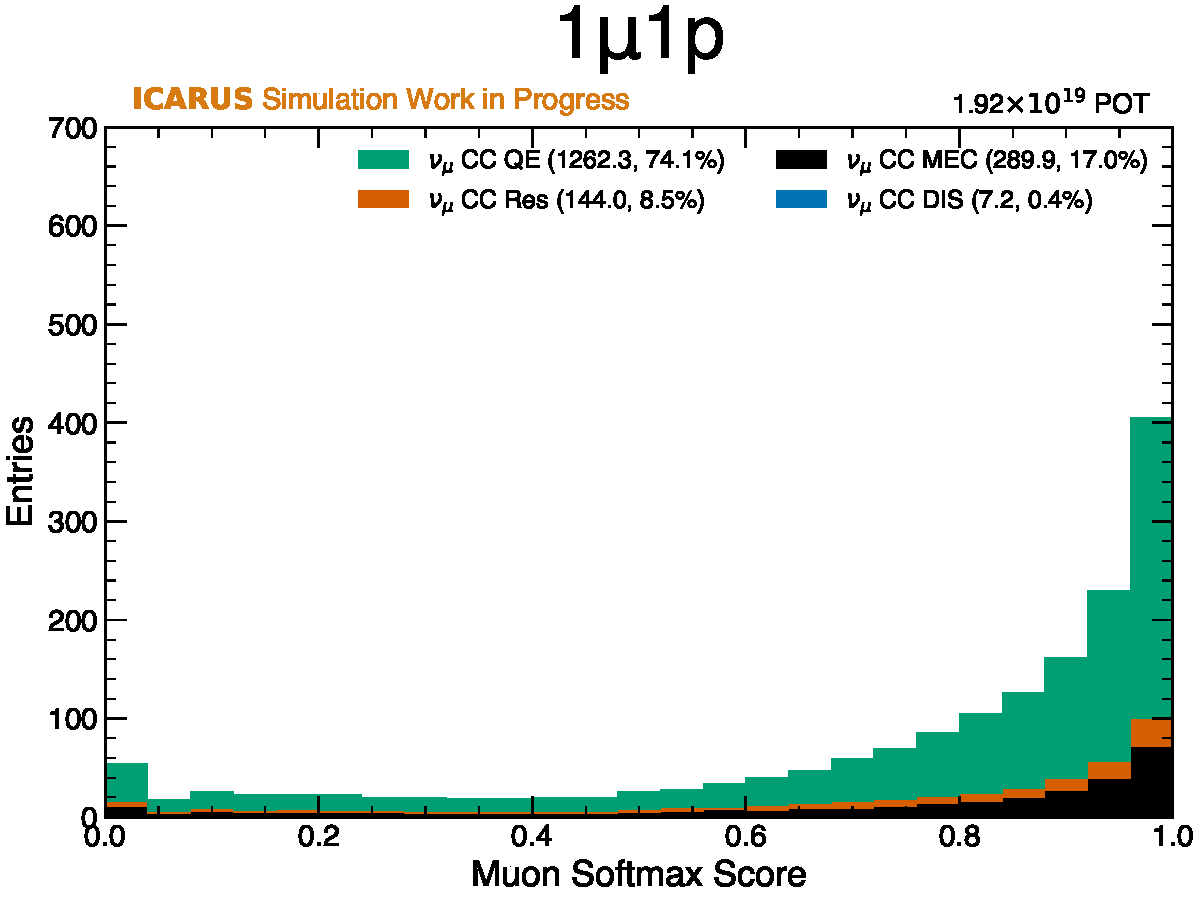
\includegraphics[width=0.48\textwidth]{figures/neutrino_selection/signal_hist1d_1mu1p_muon_softmax.pdf}
    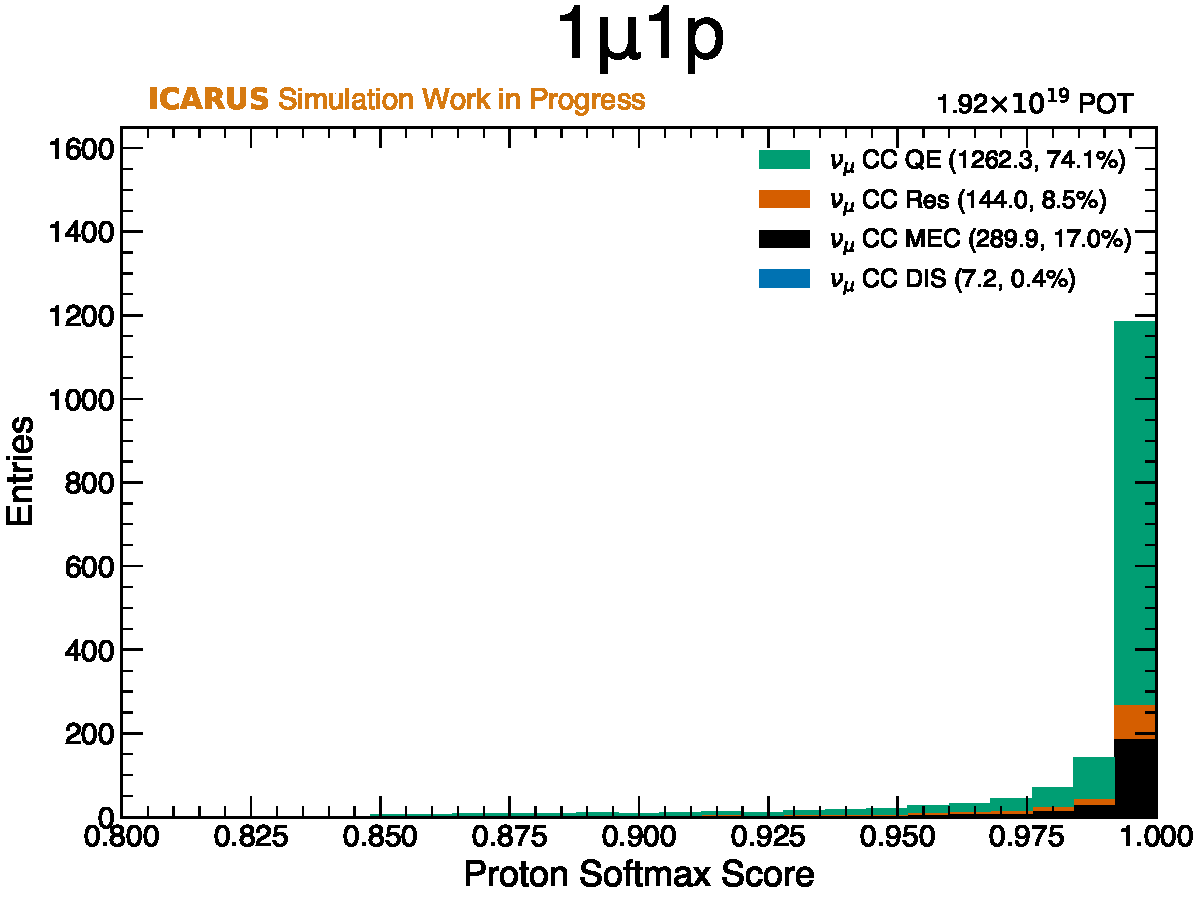
\includegraphics[width=0.48\textwidth]{figures/neutrino_selection/signal_hist1d_1mu1p_proton_softmax.pdf}
    \\
    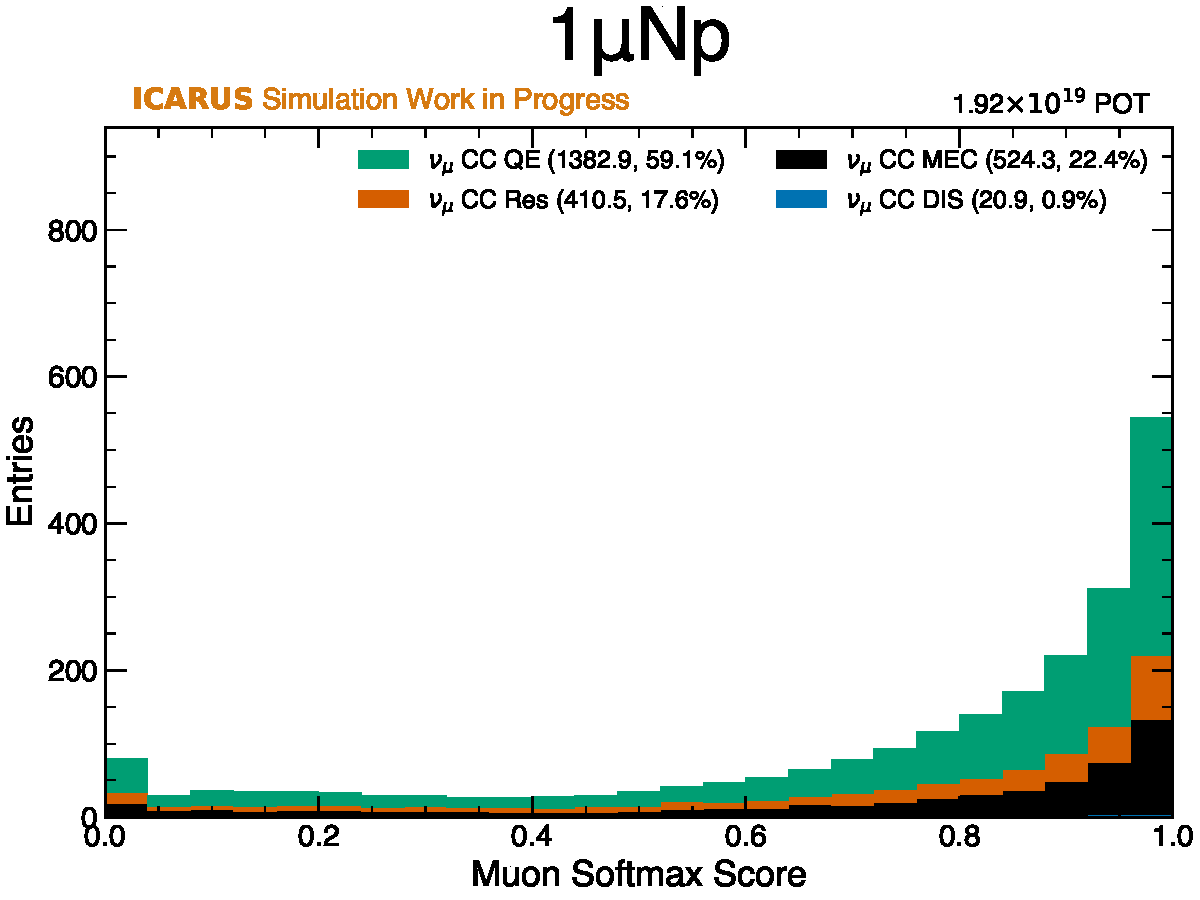
\includegraphics[width=0.48\textwidth]{figures/neutrino_selection/signal_hist1d_1muNp_muon_softmax.pdf}
    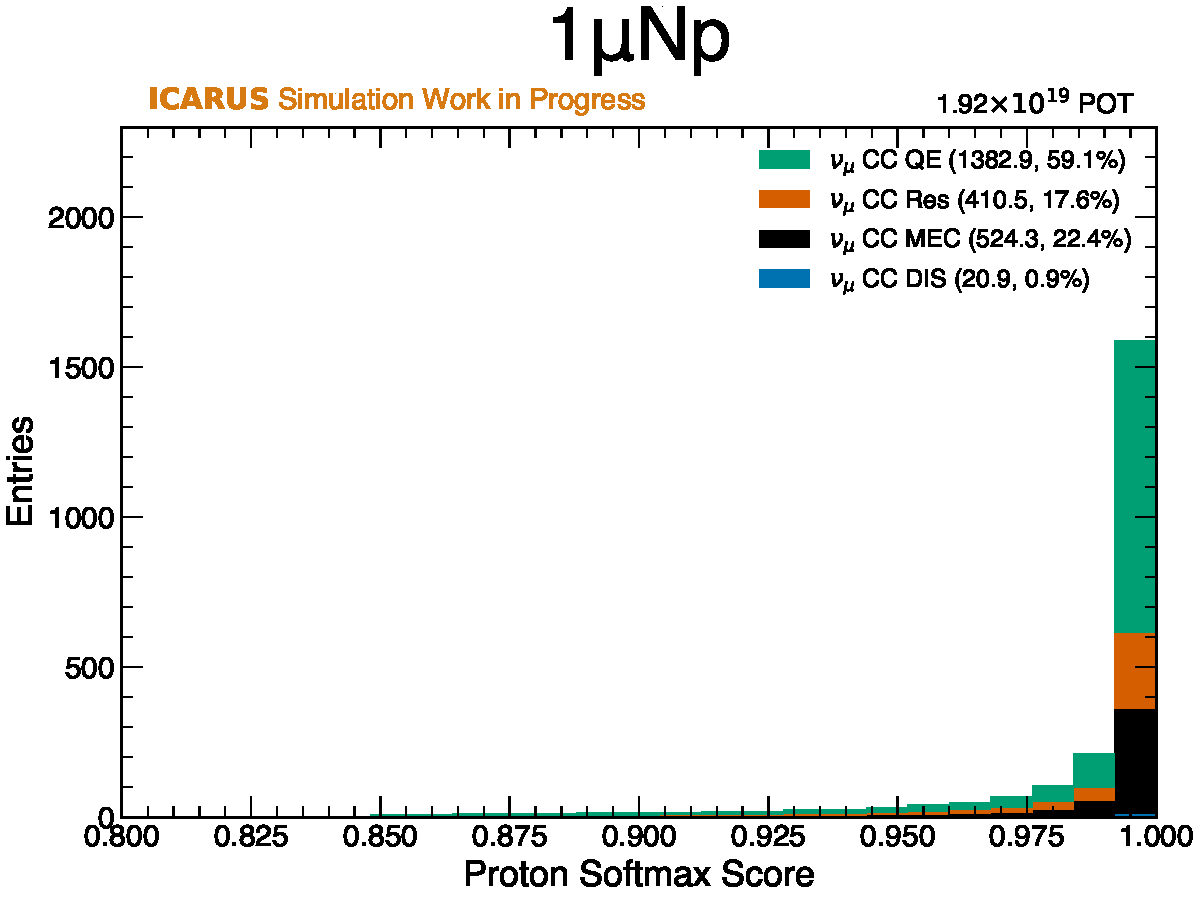
\includegraphics[width=0.48\textwidth]{figures/neutrino_selection/signal_hist1d_1muNp_proton_softmax.pdf}
    \\
    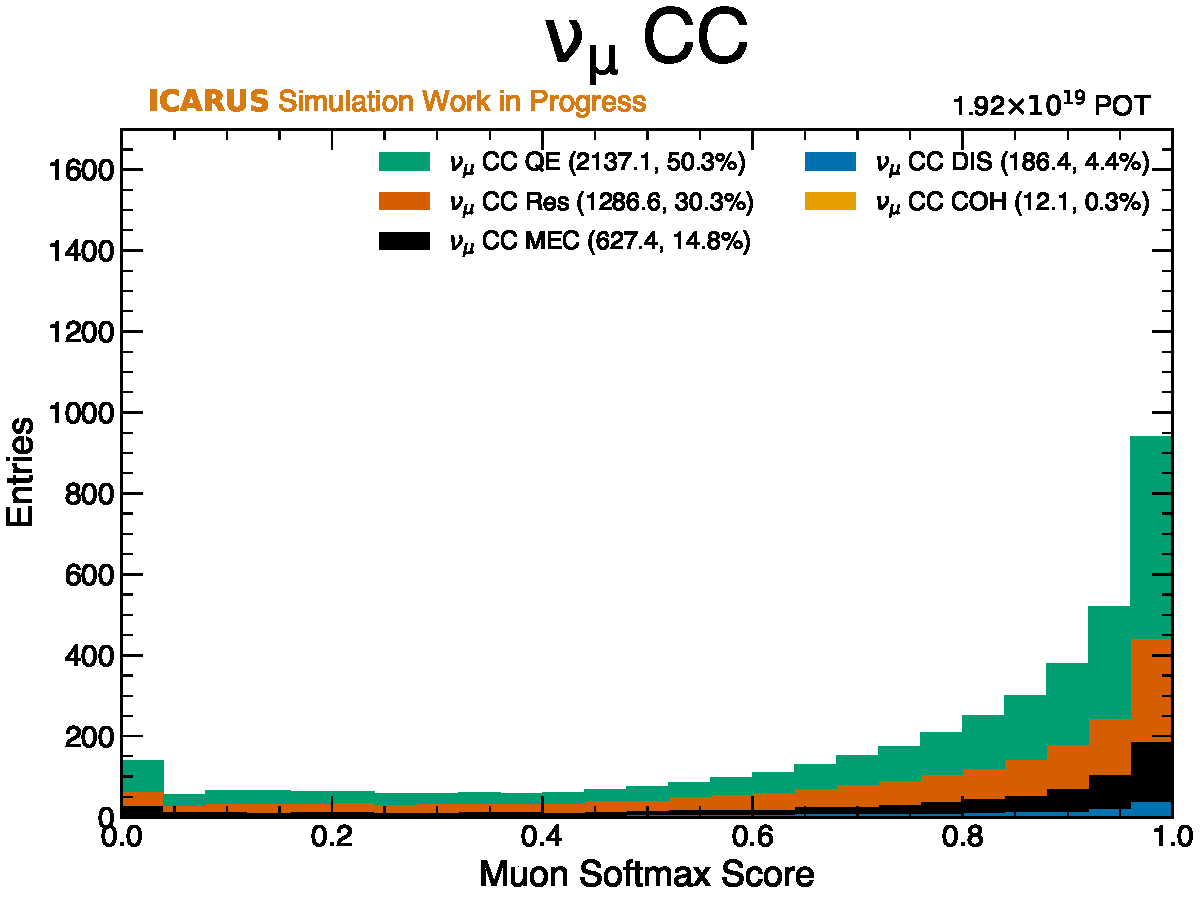
\includegraphics[width=0.48\textwidth]{figures/neutrino_selection/signal_hist1d_1muX_muon_softmax.pdf}
    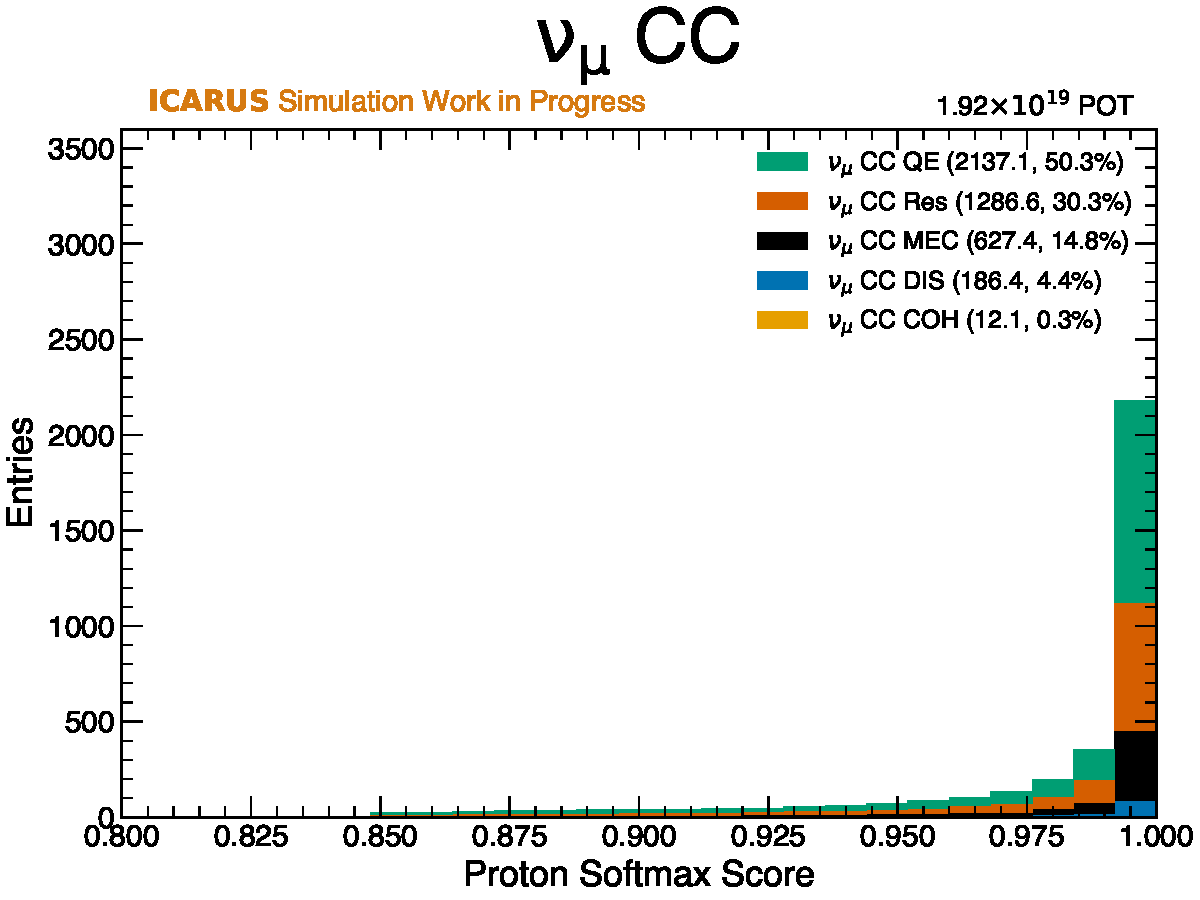
\includegraphics[width=0.48\textwidth]{figures/neutrino_selection/signal_hist1d_1muX_proton_softmax.pdf}
    \caption{Softmax PID scores for the muon candidate (left) and the leading proton candidate (right) for each of the three signal channels: from top to bottom $\mathrm{1\mu 1p}$, $\mathrm{1\mu Np}$, and $\nu_\mu$ CC inclusive.}
    \label{fig:softmax_pid}
\end{figure}

\subsection{Selection Performance}
\label{sec:selection_performance}

The performance of a selection can be characterized by its purity and efficiency. The purity of a selection is defined as the fraction of selected events that are true signal events, while the efficiency is defined as the fraction of true signal events that are selected. It is worth noting that the definition of efficiency used here is relative to the signal definition and not to the total number of neutrino interactions as may be used in other contexts. 

A table summarizing the purity and efficiency of the selections for each of the signal channels is shown in Table \ref{tab:purity_efficiency}. The purity and efficiency are calculated using the definitions described above using a Bayesian method \cite{Casadei2012} that produces more robust error bars in cases where the purity or efficiency fraction is near zero or one. Each row denotes the successive application of the selection cuts, providing a clear way to understand the impact of each cut on the purity and efficiency of the selection. From this table, several conclusions can be drawn:

\begin{table}
    \centering
    \caption{Summary of the purity and efficiency of the selections for each of the signal channels.}
    \resizebox{0.99\textwidth}{!}{\begin{tabular}{ccccccc}
\toprule
Selection Cut & $1\mu1p$ Purity [\%] & $1\mu1p$ Efficiency [\%] & $1\mu Np$ Purity [\%] & $1\mu Np$ Efficiency [\%] & $\nu_\mu$ CC Purity [\%] & $\nu_\mu$ CC Efficiency [\%] \\
\midrule
No Cut & 0.0 & 99.9 & 0.1 & 100.0 & 0.1 & 100.0 \\
Fiducial Volume & 0.1 & 98.8 & 0.1 & 98.8 & 0.3 & 98.2 \\
Containment & 1.1 & 94.9 & 1.5 & 95.0 & 3.5 & 94.1 \\
Final State & 66.2 & 73.9 & 71.2 & 77.9 & 9.5 & 86.3 \\
Flash Time & 80.1 & 72.4 & 83.0 & 76.4 & 87.8 & 84.5 \\
CRT Veto & 80.3 & 71.3 & 83.3 & 75.4 & 90.4 & 83.3 \\
\bottomrule
\end{tabular}}
    \label{tab:purity_efficiency}
\end{table}

\begin{itemize}
    \item The application of the containment cut provides a significant improvement in purity for all signal channels. This is most pronounced for the $\nu_\mu$ CC inclusive channel, where cosmic backgrounds are larger. This cut also has a non-negligible impact on the efficiency of the selection. This is largely due to cases where an un-contained cosmic-induced interaction is clustered into the neutrino interaction.
    \item The application of the cut on the final state of the candidate interactions has a significant impact on the purity of the selection for all three channels, though the impact is not as pronounced for the $\nu_\mu$ CC inclusive channel due to the presence of larger cosmic backgrounds. This is also where we see the biggest impact on the efficiency of the selection - an effect that can be directly attributed to imperfections in the reconstruction. This efficiency loss is larger for the two exclusive channels, where the final state is more constrained.
    \item The flash time cut has a negligible impact on the efficiency of the selection for all three channels, and only provides an additional improvement in purity for the $\nu_\mu$ CC inclusive channel. This is consistent with the expectation that the flash time cut primarily targets cosmic-induced interactions that are not in-time with the beam. These backgrounds are largest for the $\nu_\mu$ CC inclusive channel, which is why the impact of this cut is most pronounced for this channel.
    \item The CRT veto cut also has a $\sim$1\% impact on the efficiency of the selection for all three channels. Purity is not significantly improved except for the $\nu_\mu$ CC inclusive channel, where remaining in-time cosmic backgrounds are largest. The cost to the efficiency, though small, may not be worth it for the two exclusive channels. Since this analysis is focused on demonstrating the performance of all three selections, it is included in the final selection for all three channels to maintain consistency. It is worth highlighting that this cut may be significantly more important if the signal was extended to include interactions that exit the detector.
\end{itemize}

\begin{figure}[!htb]
    \centering
    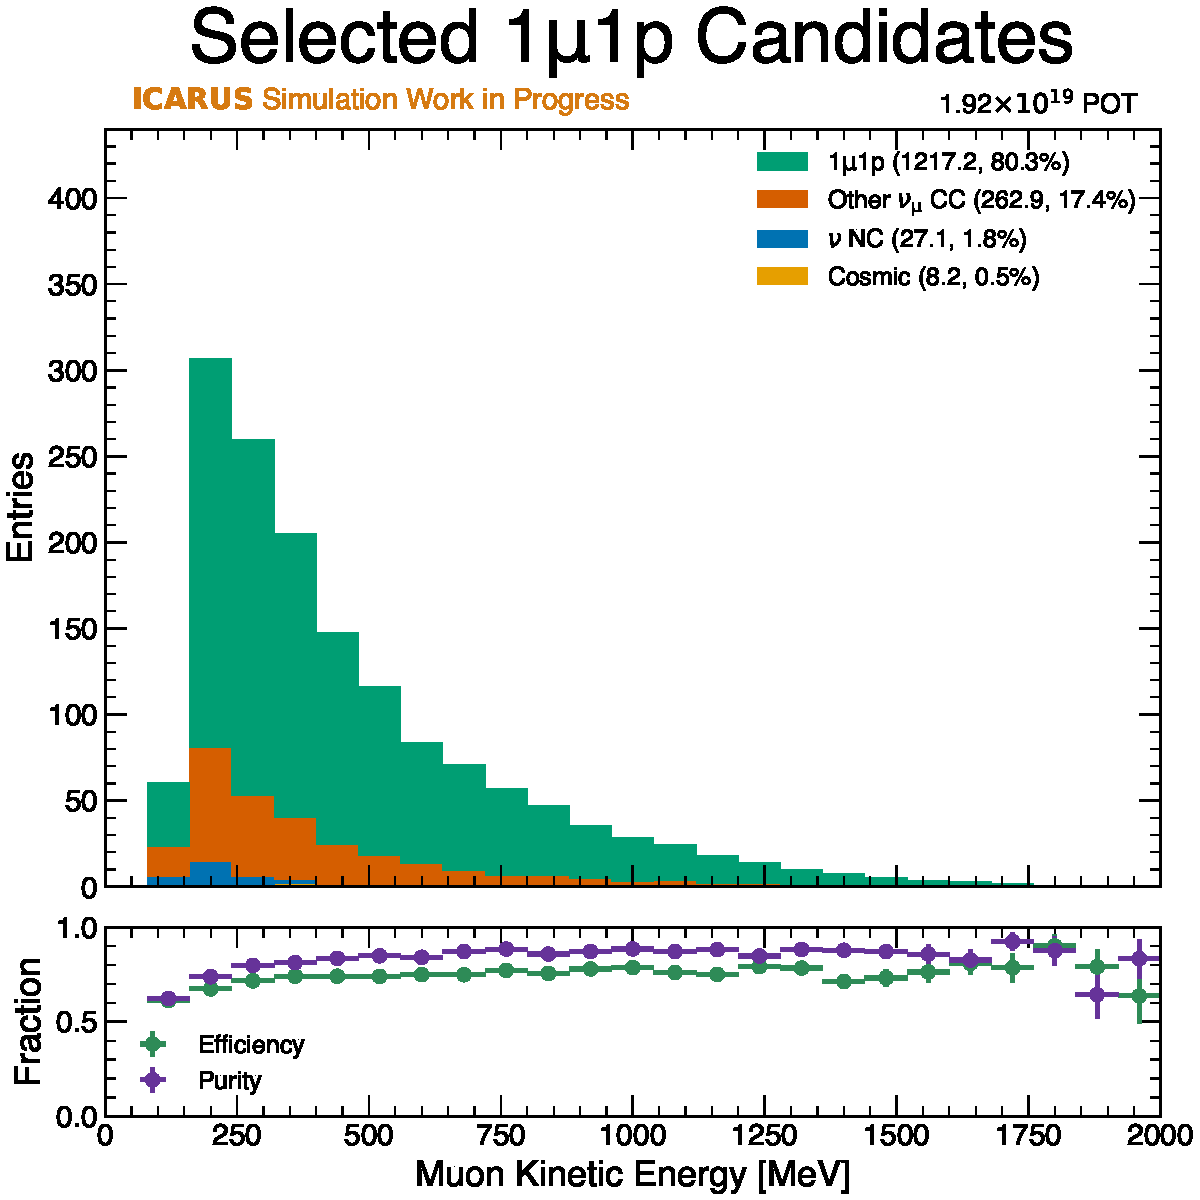
\includegraphics[width=0.42\textwidth]{figures/neutrino_selection/selected_hist1d_1mu1p_muon_ke.pdf}
    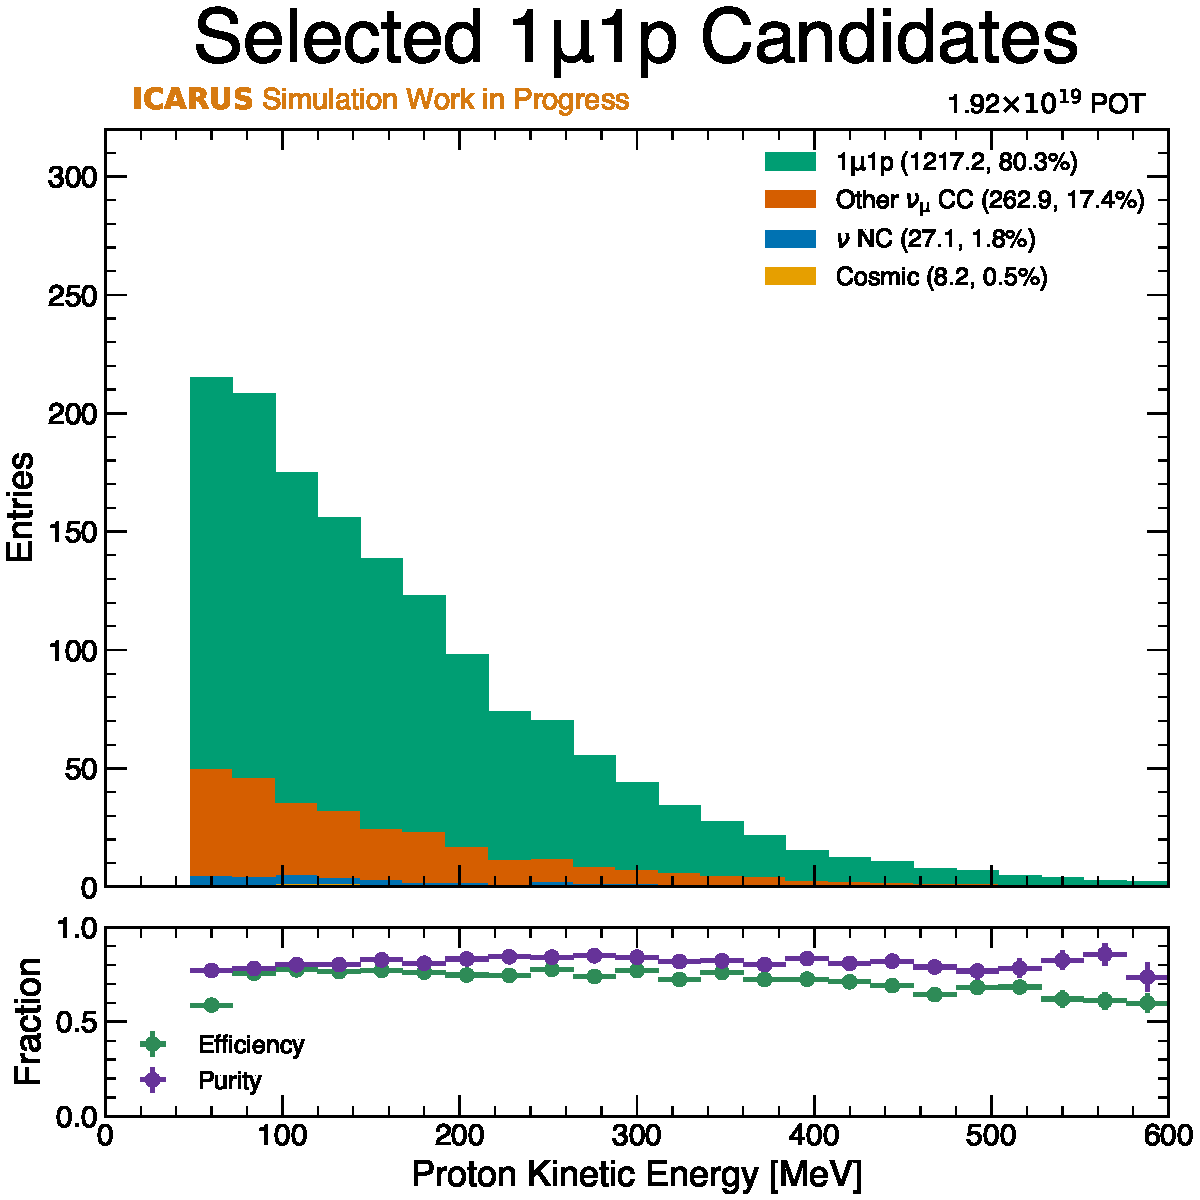
\includegraphics[width=0.42\textwidth]{figures/neutrino_selection/selected_hist1d_1mu1p_proton_ke.pdf}
    \\
    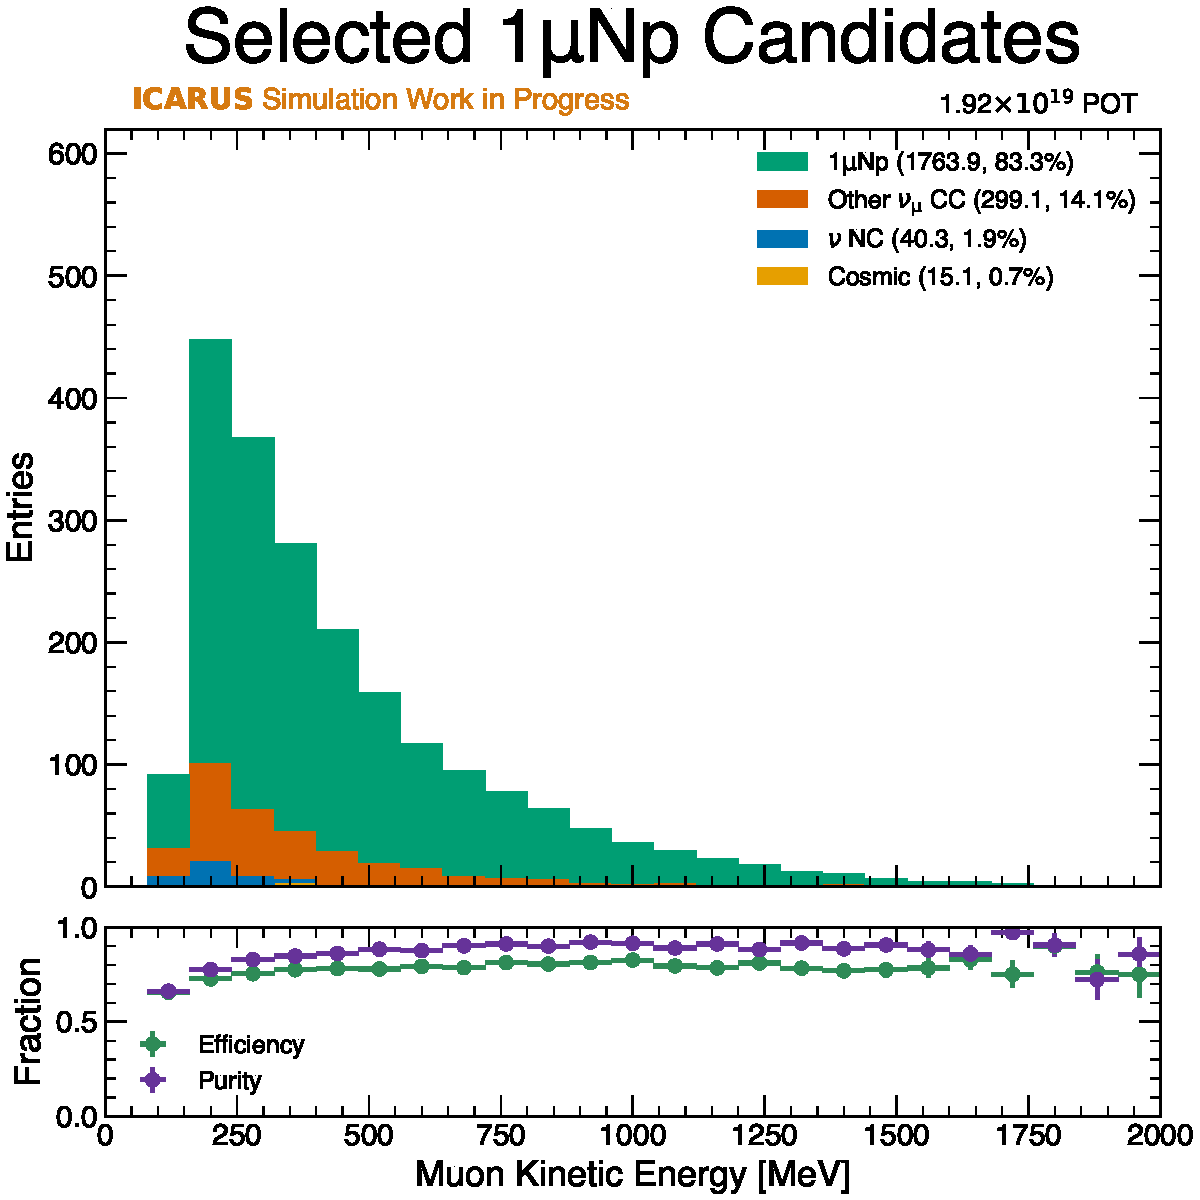
\includegraphics[width=0.42\textwidth]{figures/neutrino_selection/selected_hist1d_1muNp_muon_ke.pdf}
    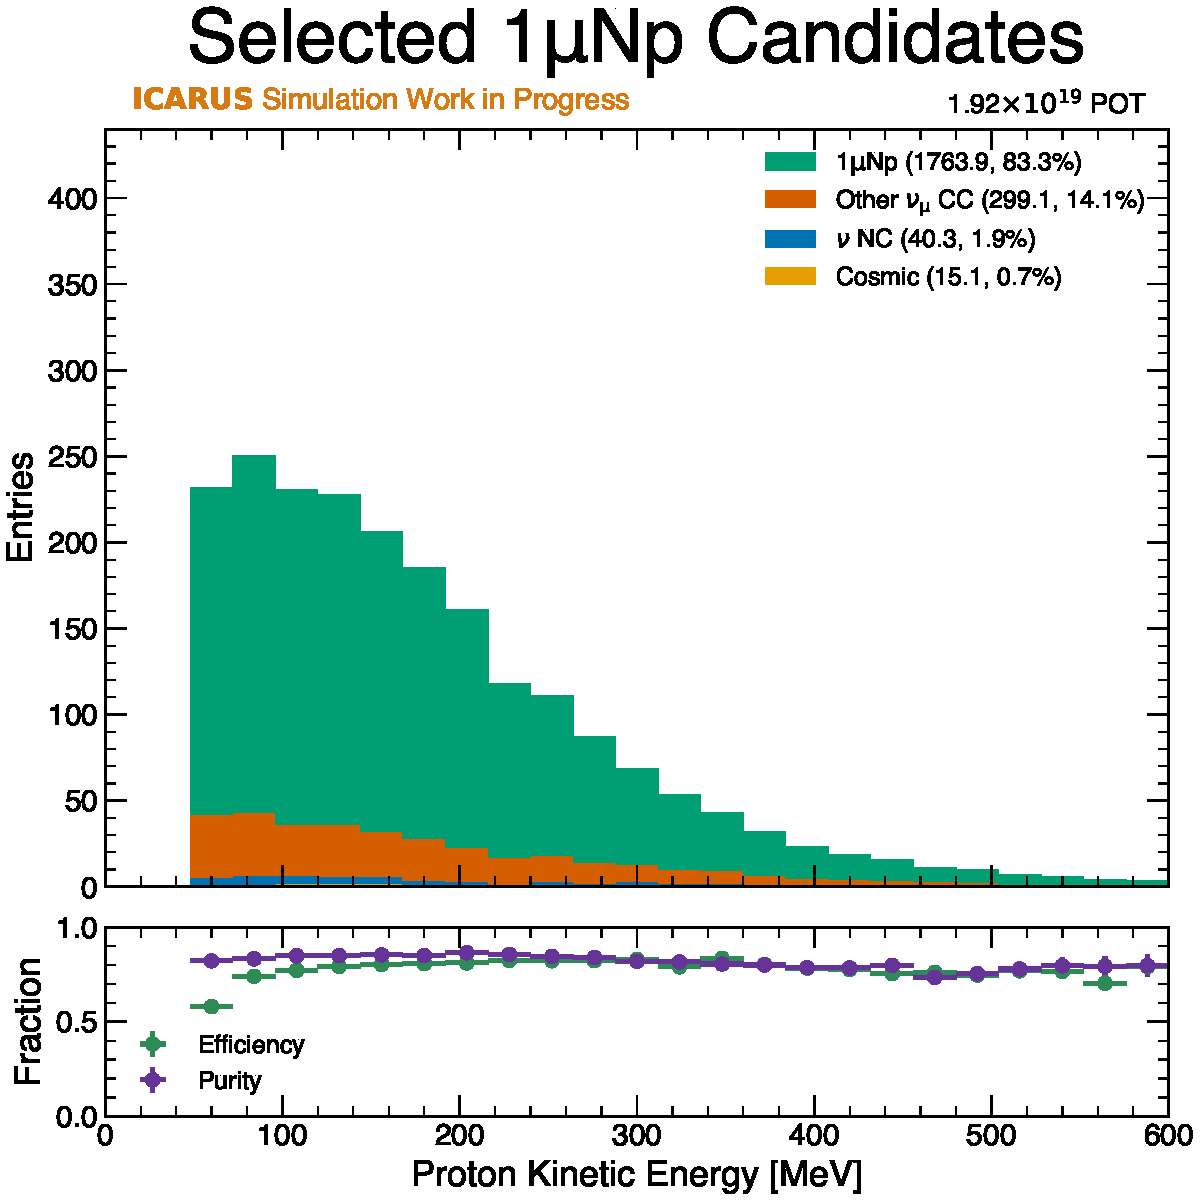
\includegraphics[width=0.42\textwidth]{figures/neutrino_selection/selected_hist1d_1muNp_proton_ke.pdf}
    \\
    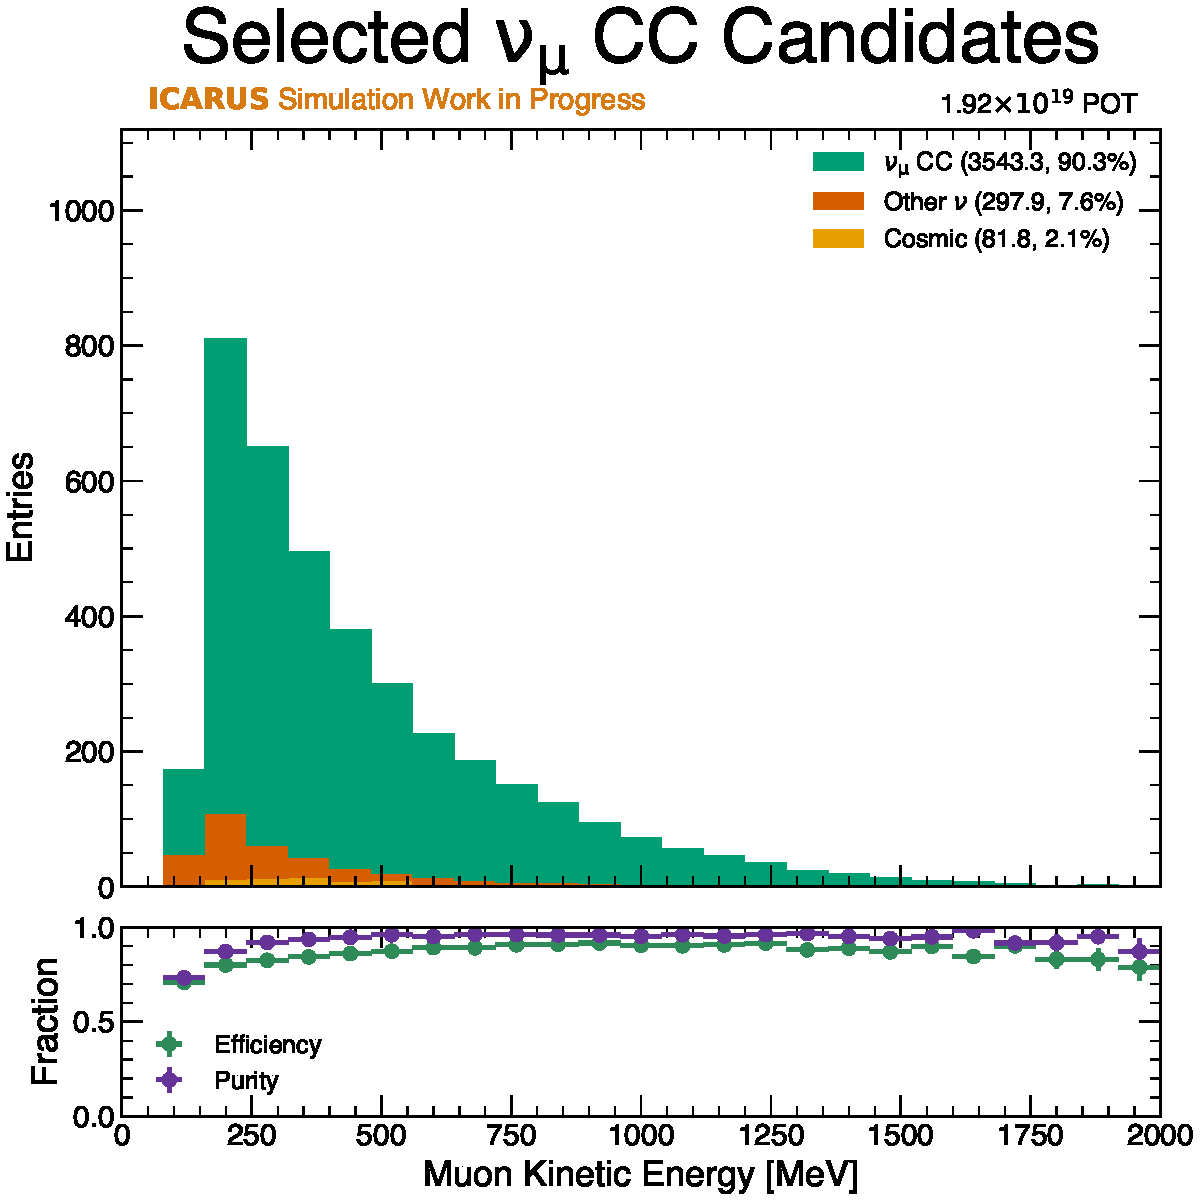
\includegraphics[width=0.42\textwidth]{figures/neutrino_selection/selected_hist1d_1muX_muon_ke.pdf}
    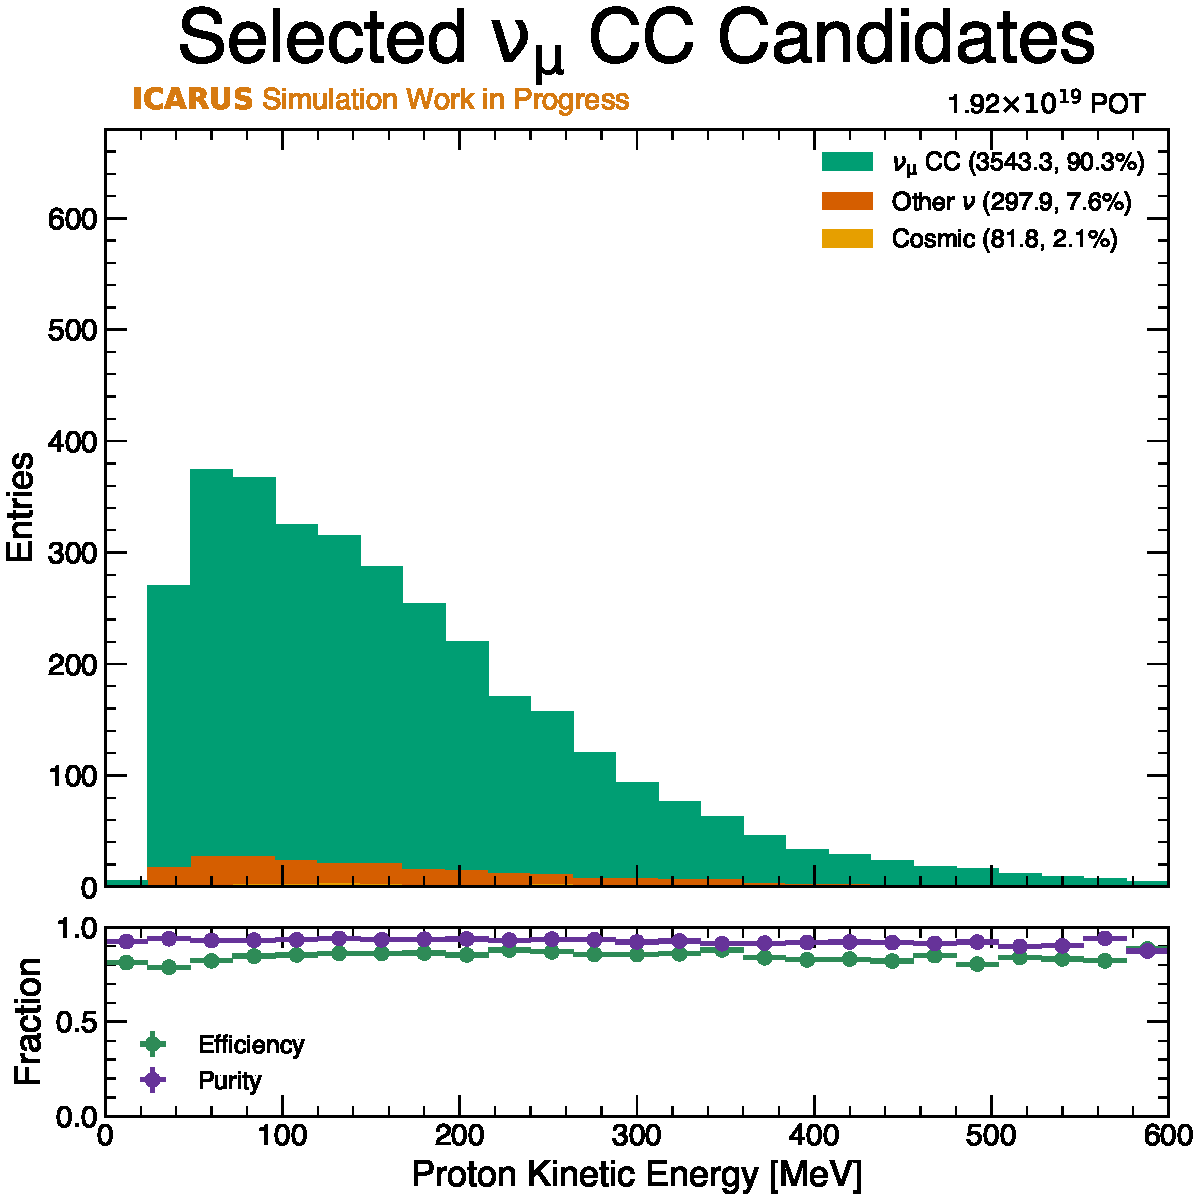
\includegraphics[width=0.42\textwidth]{figures/neutrino_selection/selected_hist1d_1muX_proton_ke.pdf}
    \caption{Purity and efficiency as a function of the kinetic energy of the muon (left) and the most energetic proton (right) for each of the three signal channels: from top to bottom $\mathrm{1\mu 1p}$, $\mathrm{1\mu Np}$, and $\nu_\mu$ CC inclusive.}
    \label{fig:pureff_muon_proton_ke}
\end{figure}

\begin{figure}[!htb]
    \centering
    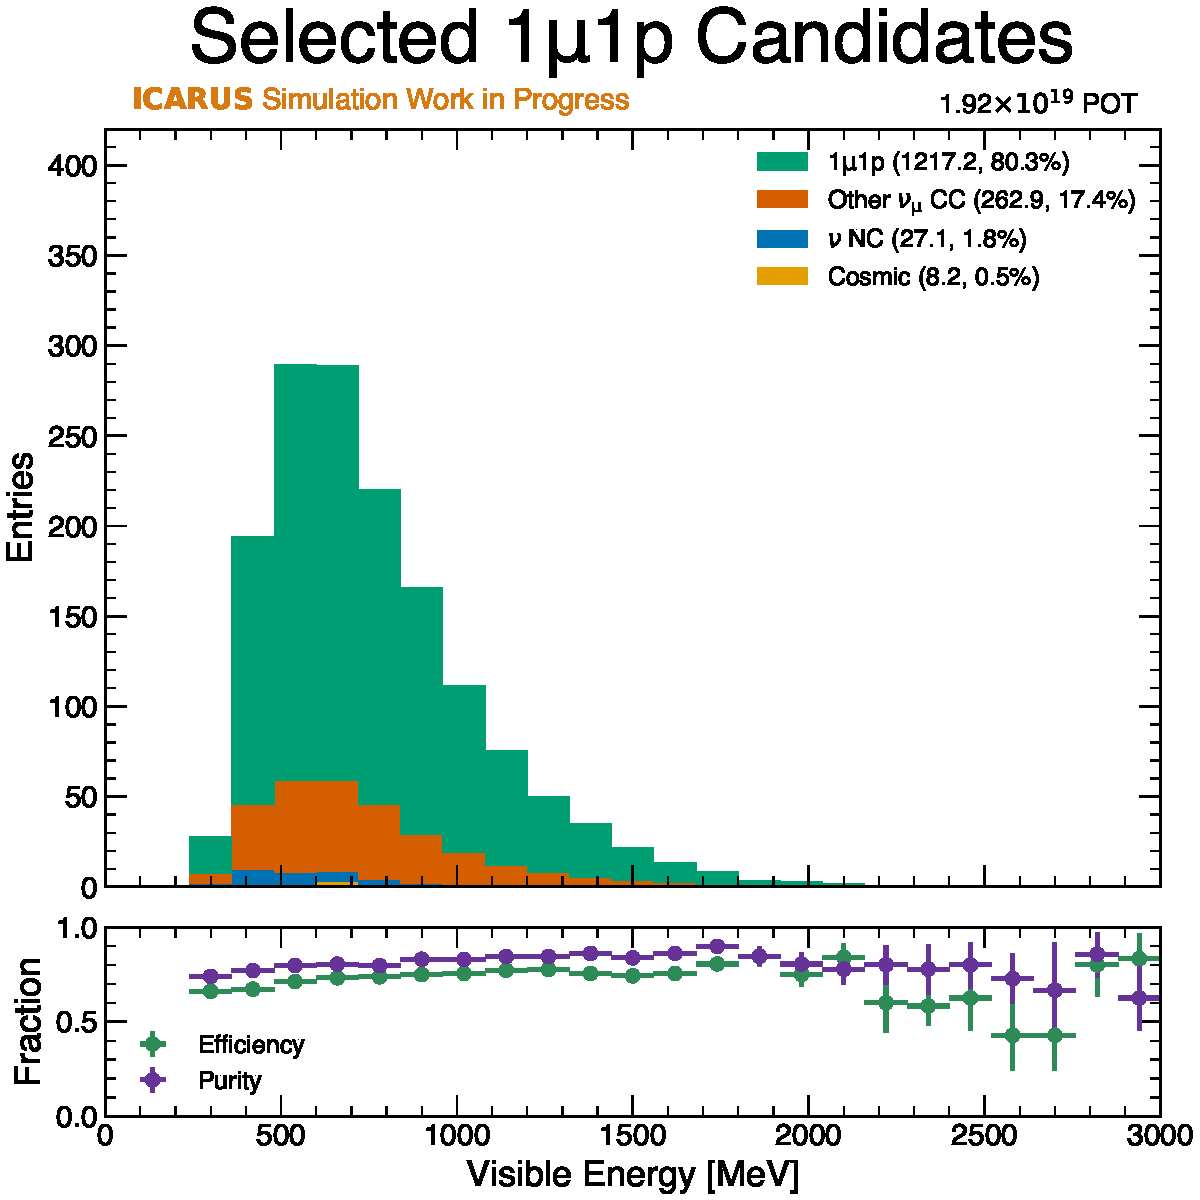
\includegraphics[width=0.42\textwidth]{figures/neutrino_selection/selected_hist1d_1mu1p_visible_energy.pdf}\\
    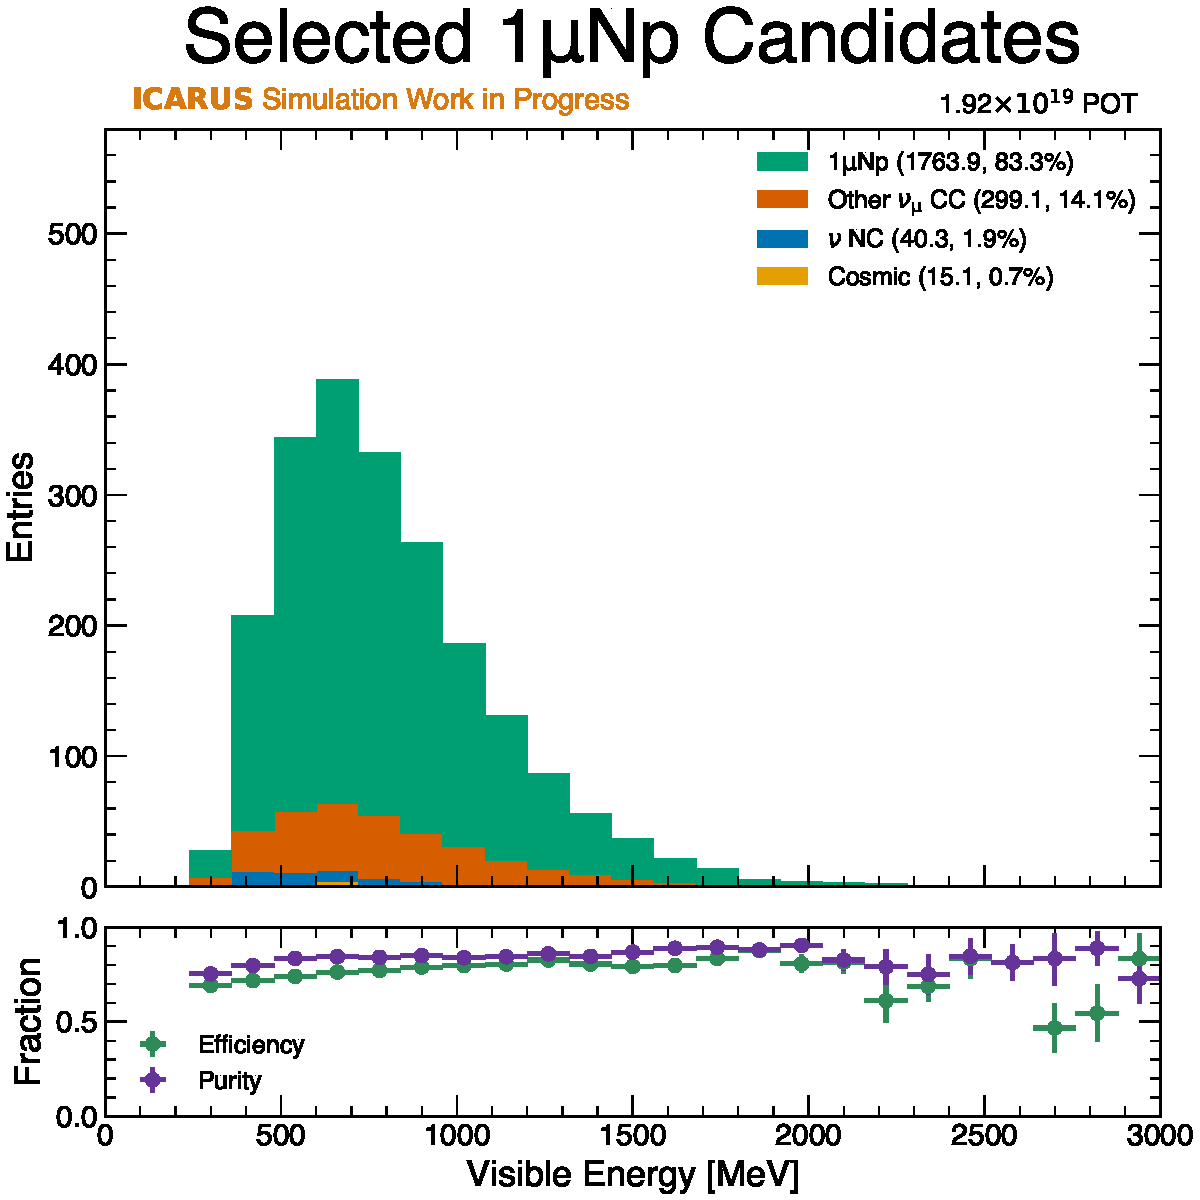
\includegraphics[width=0.42\textwidth]{figures/neutrino_selection/selected_hist1d_1muNp_visible_energy.pdf}\\
    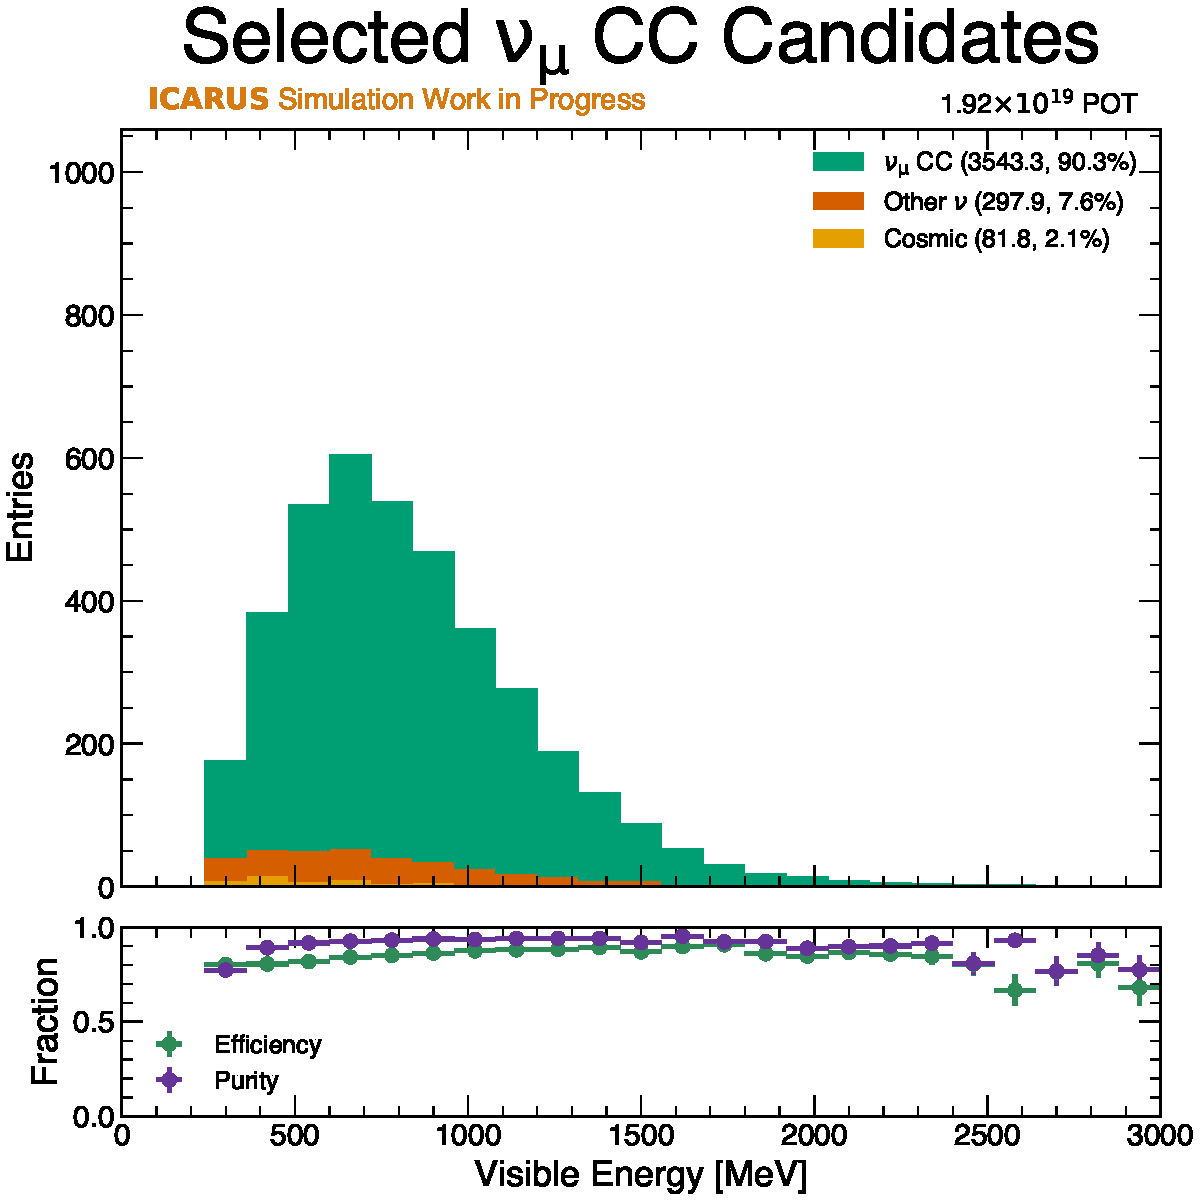
\includegraphics[width=0.42\textwidth]{figures/neutrino_selection/selected_hist1d_1muX_visible_energy.pdf}\\
    \caption{Purity and efficiency as a function of the total visible energy of the interaction for each of the signal channels: from top to bottom $\mathrm{1\mu 1p}$, $\mathrm{1\mu Np}$, and $\nu_\mu$ CC inclusive.}
    \label{fig:pureff_visible_energy}
\end{figure}

\begin{figure}[!htb]
    \centering
    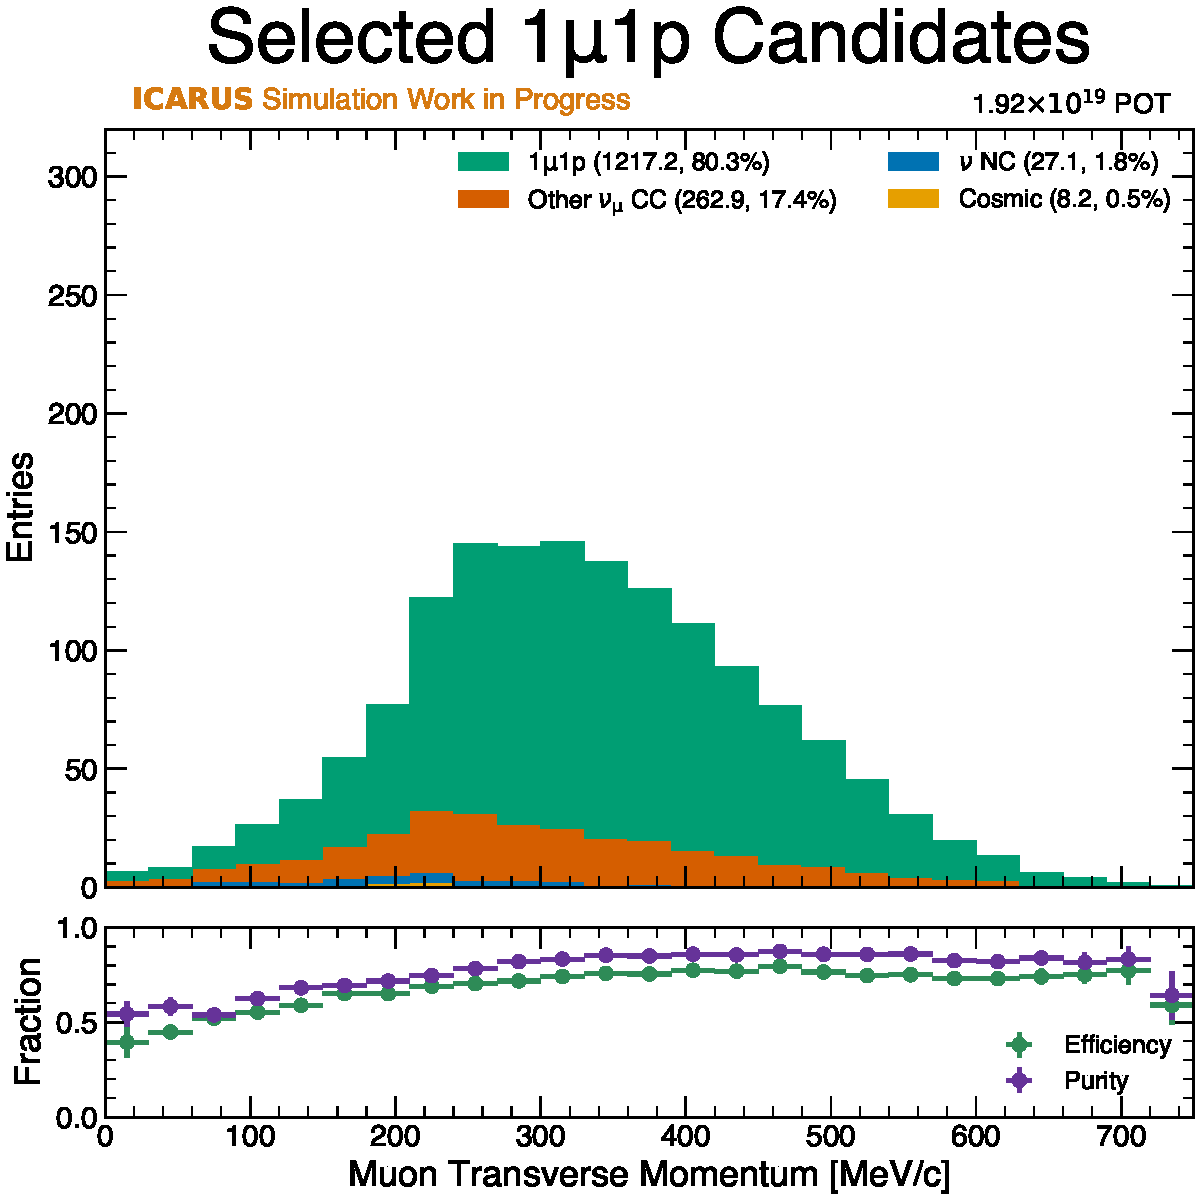
\includegraphics[width=0.41\textwidth]{figures/neutrino_selection/selected_hist1d_1mu1p_muon_pt.pdf}
    \includegraphics[width=0.41\textwidth]{figures/neutrino_selection/selected_hist1d_1mu1p_proton_pt.pdf}
    \\
    \includegraphics[width=0.41\textwidth]{figures/neutrino_selection/selected_hist1d_1muNp_muon_pt.pdf}
    \includegraphics[width=0.41\textwidth]{figures/neutrino_selection/selected_hist1d_1muNp_proton_pt.pdf}
    \\
    \includegraphics[width=0.41\textwidth]{figures/neutrino_selection/selected_hist1d_1muX_muon_pt.pdf}
    \includegraphics[width=0.41\textwidth]{figures/neutrino_selection/selected_hist1d_1muX_proton_pt.pdf}
    \caption{Purity and efficiency as a function of the transverse momentum of the muon (left) and the most energetic proton (right) for each of the three signal channels: from top to bottom $\mathrm{1\mu 1p}$, $\mathrm{1\mu Np}$, and $\nu_\mu$ CC inclusive. The peak at the lowest bin in the inclusive channel in the proton transverse momentum variable is from interactions where no proton is present.}
    \label{fig:pureff_muon_proton_pt}
\end{figure}

\begin{figure}[!htb]
    \centering
    \includegraphics[width=0.42\textwidth]{figures/neutrino_selection/selected_hist1d_1mu1p_muon_polar_angle.pdf}
    \includegraphics[width=0.42\textwidth]{figures/neutrino_selection/selected_hist1d_1mu1p_muon_azimuthal_angle.pdf}
    \\
    \includegraphics[width=0.42\textwidth]{figures/neutrino_selection/selected_hist1d_1muNp_muon_polar_angle.pdf}
    \includegraphics[width=0.42\textwidth]{figures/neutrino_selection/selected_hist1d_1muNp_muon_azimuthal_angle.pdf}
    \\
    \includegraphics[width=0.42\textwidth]{figures/neutrino_selection/selected_hist1d_1muX_muon_polar_angle.pdf}
    \includegraphics[width=0.42\textwidth]{figures/neutrino_selection/selected_hist1d_1muX_muon_azimuthal_angle.pdf}
    \caption{Purity and efficiency as a function of the polar angle (left) and azimuthal angle (right) of the muon for each of the three signal channels: from top to bottom $\mathrm{1\mu 1p}$, $\mathrm{1\mu Np}$, and $\nu_\mu$ CC inclusive.}
    \label{fig:pureff_muon_angles}
\end{figure}

\begin{figure}[!htb]
    \centering
    \includegraphics[width=0.42\textwidth]{figures/neutrino_selection/selected_hist1d_1mu1p_opening_angle.pdf}\\
    \includegraphics[width=0.42\textwidth]{figures/neutrino_selection/selected_hist1d_1muNp_opening_angle.pdf}\\
    \includegraphics[width=0.42\textwidth]{figures/neutrino_selection/selected_hist1d_1muX_opening_angle.pdf}\\
    \caption{Purity and efficiency as a function of the the muon-proton opening angle for each of the three signal channels: from top to bottom $\mathrm{1\mu 1p}$, $\mathrm{1\mu Np}$, and $\nu_\mu$ CC inclusive.}
    \label{fig:pureff_opening_angle}
\end{figure}

\begin{figure}[!htb]
    \centering
    \includegraphics[width=0.42\textwidth]{figures/neutrino_selection/selected_hist1d_1mu1p_delta_pT.pdf}\\
    \includegraphics[width=0.42\textwidth]{figures/neutrino_selection/selected_hist1d_1muNp_delta_pT.pdf}\\
    \includegraphics[width=0.42\textwidth]{figures/neutrino_selection/selected_hist1d_1muX_delta_pT.pdf}\\
    \caption{Purity and efficiency as a function of the transverse momentum of the interaction for each of the three signal channels: from top to bottom $\mathrm{1\mu 1p}$, $\mathrm{1\mu Np}$, and $\nu_\mu$ CC inclusive.}
    \label{fig:pureff_delta_pT}
\end{figure}

\begin{figure}[!htb]
    \centering
    \includegraphics[width=0.42\textwidth]{figures/neutrino_selection/selected_hist1d_1mu1p_delta_alphaT.pdf}
    \includegraphics[width=0.42\textwidth]{figures/neutrino_selection/selected_hist1d_1mu1p_delta_phiT.pdf}
    \\
    \includegraphics[width=0.42\textwidth]{figures/neutrino_selection/selected_hist1d_1muNp_delta_alphaT.pdf}
    \includegraphics[width=0.42\textwidth]{figures/neutrino_selection/selected_hist1d_1muNp_delta_phiT.pdf}
    \\
    \includegraphics[width=0.42\textwidth]{figures/neutrino_selection/selected_hist1d_1muX_delta_alphaT.pdf}
    \includegraphics[width=0.42\textwidth]{figures/neutrino_selection/selected_hist1d_1muX_delta_phiT.pdf}
    \caption{Purity and efficiency as a function of the kinematic imbalance variables $\delta \alpha_T$ (left) and $\delta \phi_T$ (right) for each of the three signal channels: from top to bottom $\mathrm{1\mu 1p}$, $\mathrm{1\mu Np}$, and $\nu_\mu$ CC inclusive.}
    \label{fig:pureff_kinematic_imbalance_angles}
\end{figure}

The purity and efficiency of a selection can also be visualized as a function of the variables of interest to understand the relationship between the selection and each variable. This can help to identify regions of phase space where the selection is particularly efficient or pure, and to identify regions where the selection may be underperforming. In each of the following plots, the purity and efficiency are calculated per-bin using the same binning as the variable itself. The selected candidates are binned according to the \textit{reconstructed} variable, as opposed to the true quantity presented previously, and broken down into categories based on their true final state. These plots are shown in Figures \ref{fig:pureff_muon_proton_ke} through \ref{fig:pureff_kinematic_imbalance_angles}. There are several notable features worth highlighting:

\begin{itemize}
    \item Generally, the purity and efficiency drop off at regions of phase space correlated with lower energy. Smaller particles are more likely to be mis-reconstructed and may not be as separable from other particles in the final state. 
    \item Angles where tracks are parallel to the wire planes are more likely to be mis-reconstructed. This is especially visible in the muon and proton transverse momentum variables, where the lower values are associated with a particle that is more aligned with the $z$-axis. This is a known side effect of the coherent noise filtering algorithm used upstream in the reconstruction chain, which tends to remove signal from tracks that are parallel to the wire planes.
    \item There is a drop in purity and efficiency for the two exclusive channels at higher values of the muon-proton opening angle. This is due to the difficulty in separating the muon and proton tracks when they are highly collinear.
    \item The values of $\delta p_T$ outside of the Fermi momentum are associated with a drop in purity and efficiency for the two exclusive channels. This is a region of phase space with fewer QE interactions and more complex interactions that are more difficult to reconstruct.
\end{itemize}

At this stage of the analysis, the selections are performing well in terms of purity and efficiency on simulation. Benchmarking the performance of the selections on data is a key step in the validation of the selections and the reconstruction chain, but prior to this step the full set of uncertainties must be understood. This will be the focus of the next chapter.

